% !TeX root = digital-platform-api-economy.tex
% !TeX encoding = UTF-8
\chapter{Tata Kelola API dan Regulasi Platform}
\label{ch:ch13}

% Kolom rata kiri untuk tabel bab ini: G selebar sisa tabel, H selebar yang ditentukan.
\newcolumntype{G}{>{\raggedright\arraybackslash}X}
\newcolumntype{H}[1]{>{\raggedright\arraybackslash}p{#1}}
\lstdefinestyle{ch13yaml}{language=yaml, basicstyle=\ttfamily\scriptsize, morestring=[b]', captionpos=b, xleftmargin=8pt,
  columns=fullflexible, keepspaces=true}

\section*{Tujuan Pembelajaran}
\begin{itemize}
  \item Merancang model tata kelola API yang menjaga konsistensi tanpa memperlambat tim.
  \item Menjelaskan risiko persaingan usaha pada platform beserta regulasinya di Indonesia dan Uni Eropa.
  \item Menilai batasan regulasi terhadap rancangan platform organisasi.
\end{itemize}

\section{Pendahuluan}

Lima rumah sakit Medikara berasal dari akuisisi, sehingga kebiasaan penamaan dan keputusan \textit{Application Programming
Interface} (API) di dalamnya berbeda. Menyeragamkan seluruh keputusan di pusat menciptakan antrean. Membebaskan semuanya
memperbesar ketidakkonsistenan. Bab sebelumnya sudah menghasilkan banyak keputusan: 20 sambungan aktif dengan biaya Rp45 juta
per antarmuka, delapan kandidat API-01 sampai API-08, kontrak API-01, masa transisi 6 bulan, \textit{Service Level Agreement}
(SLA) 99,0 persen dengan \textit{Service Level Objective} (SLO) 99,4 persen, serta paket berjenjang untuk 40 klinik mitra.
Pertanyaan kemudian muncul: siapa berwenang mengubah semua itu, dan batas apa yang tidak boleh diputuskan sendiri oleh Medikara?

Bab ini menjawabnya dalam dua bagian. Bagian pertama membahas tata kelola di dalam organisasi: model keputusan, panduan gaya,
tinjauan, pemeriksaan otomatis, katalog, dan aturan bagi mitra. Bagian kedua membahas batas dari luar organisasi: persaingan usaha,
\textit{Digital Markets Act} (DMA) Uni Eropa, pelindungan data, dan aturan sektor kesehatan. Kedua bagian bertemu pada posisi
Medikara yang mengatur Medikara+, sekaligus memiliki 18 klinik dan 12 apotek yang bersaing dengan mitra. Angka tambahan yang diawali
kata ``Misalkan'' adalah asumsi latihan. Kesimpulan untuk organisasi nyata harus diuji dengan wawancara, dokumen, pengukuran yang
berizin, dan penasihat hukum. Bab ini bukan nasihat hukum. COBIT, manajemen risiko, dan Undang-Undang Pelindungan Data Pribadi (UU PDP)
secara umum dibahas rinci di IT40813. Hasil bab ini menjadi bagian C4 dalam cetak biru transformasi digital.

Rujukan utama bab ini dipakai untuk membedakan konsep dan membangun alasan keputusan, bukan untuk menggantikan penilaian konteks
organisasi. Tata kelola API mengikuti Medjaoui dkk. \cite{medjaoui2021continuous}, sedangkan tata kelola platform mengikuti Tiwana dan
rekan \cite{tiwana2010platform, tiwana2014platform}. Batas hukum memakai Undang-Undang (UU) 5/1999 \cite{uu5-1999-persaingan},
perkara Komisi Pengawas Persaingan Usaha (KPPU) tentang Google Play Billing \cite{c13-kppu-google2025}, DMA \cite{eu-dma-2022}, UU 27/2022
\cite{uu27-2022-pdp}, dan Peraturan Pemerintah (PP) 33/2026 \cite{c13-pp33-2026}. Sumber yang belum dapat dicocokkan ke teks resmi ditandai
langsung pada kalimat atau tabel yang memakainya.

\IfFileExists{../figures/ch13-diagram-konsep.png}{%

Gambar \ref{fig:ch13-ilustrasi-bab} merangkum hubungan komponen dan konsep utama bab ini.
\begin{figure}[!htb]
  \centering
  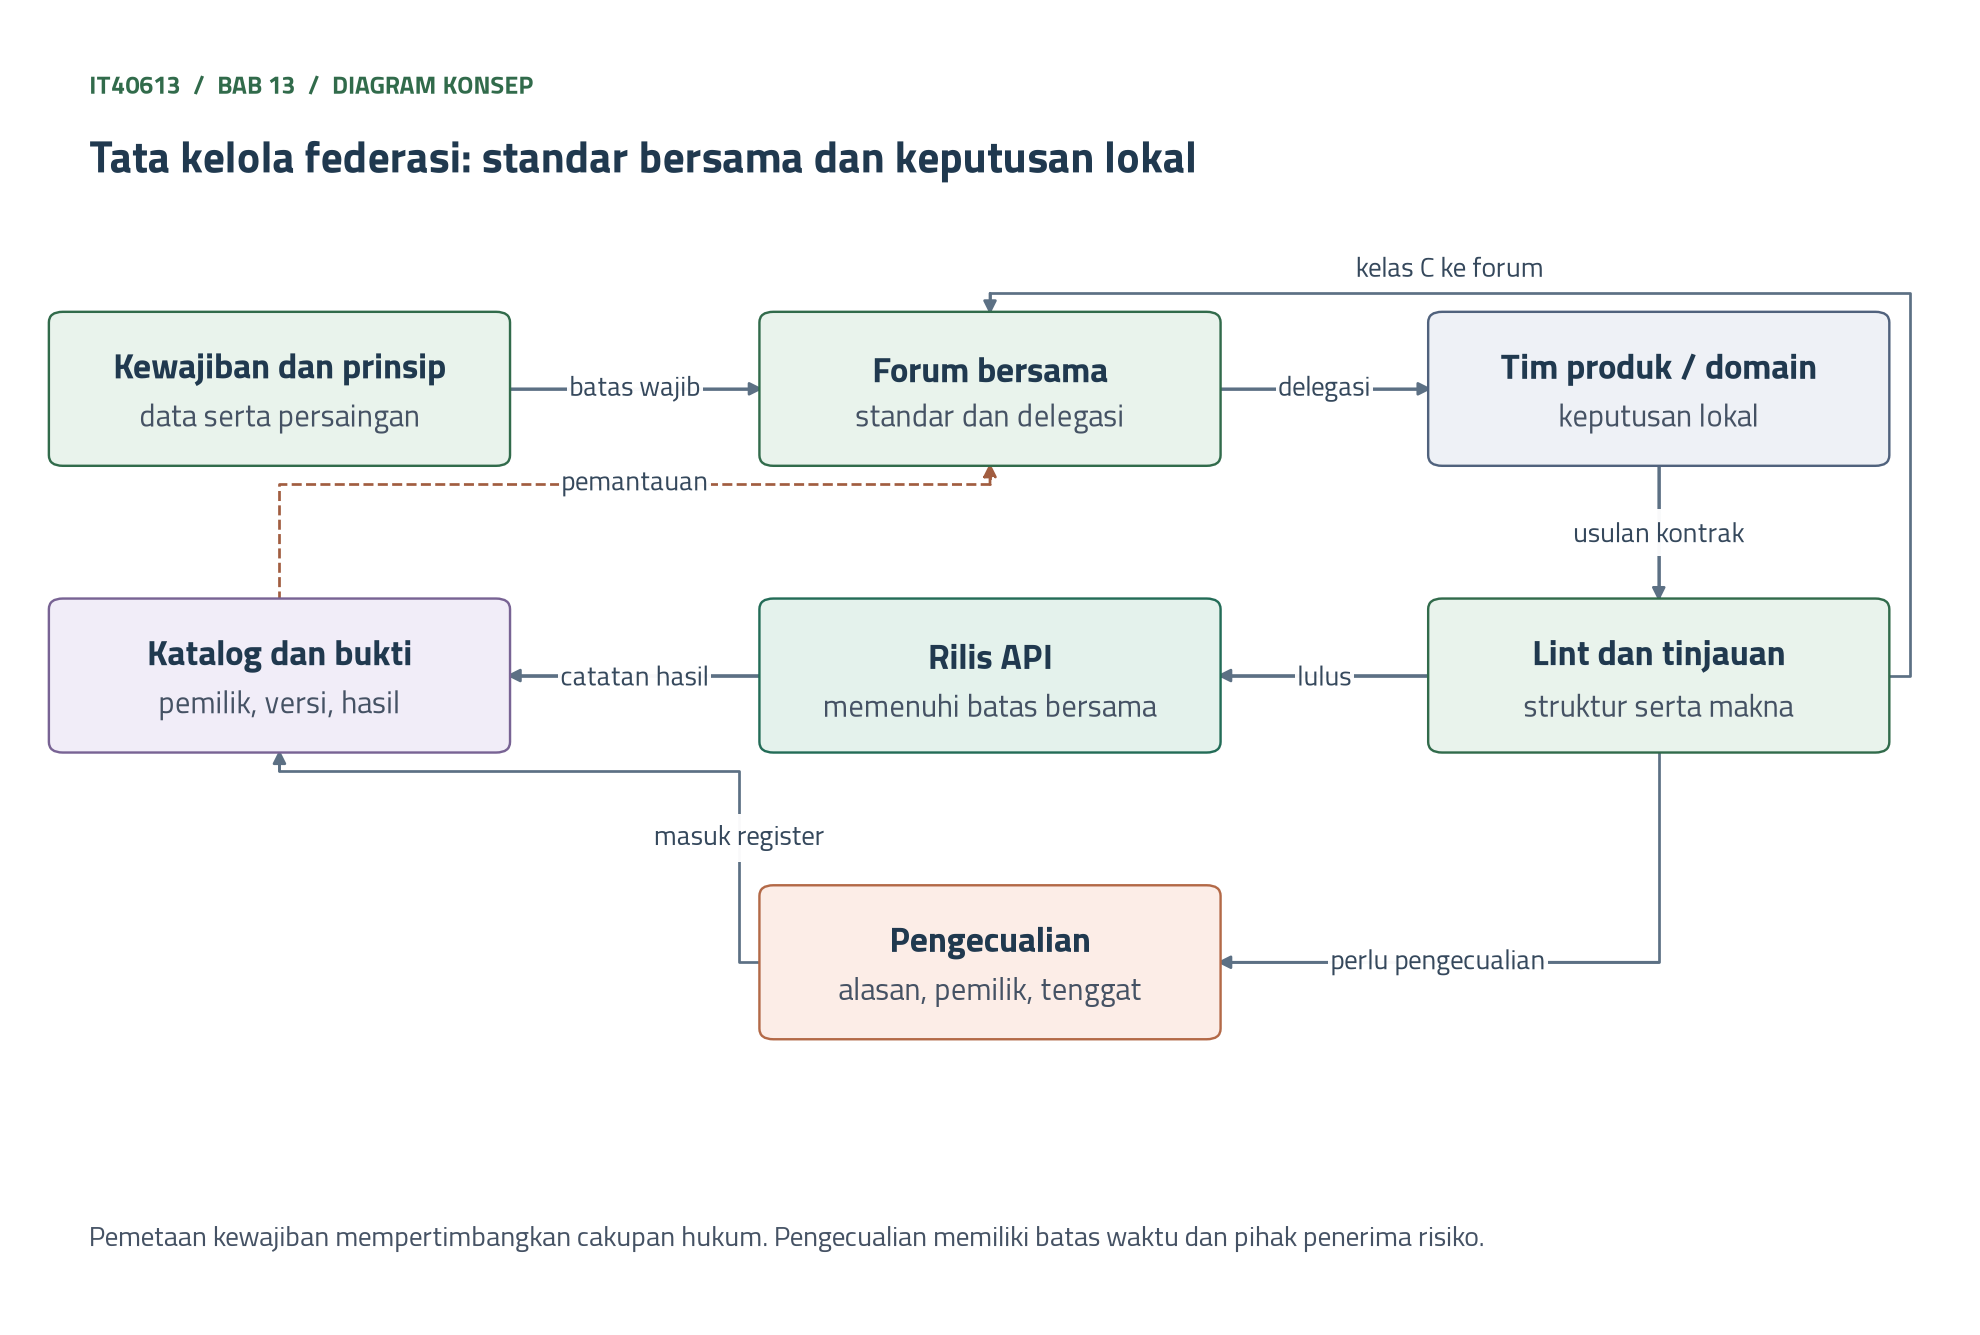
\includegraphics[width=\textwidth]{../figures/ch13-diagram-konsep.png}
  \caption{Tata kelola federasi: standar bersama dan keputusan lokal}
  \label{fig:ch13-ilustrasi-bab}
\end{figure}
}{}

\section{Tata Kelola API sebagai Pemungkin}

Mengapa organisasi yang ingin bergerak cepat justru memerlukan aturan? Jawabannya ada pada biaya berunding ulang. Tim bergerak lebih
cepat bila tidak perlu memperdebatkan hal yang sama pada setiap API.

Tata kelola API menetapkan hak keputusan, standar minimum, bukti persetujuan, dan cara menangani pengecualian. Tujuannya menjaga
kemampuan organisasi melakukan perubahan dengan konsisten. Pemeriksaan disesuaikan dengan risiko, sehingga perubahan kecil tidak
memerlukan forum yang sama dengan pembukaan data sensitif kepada mitra. Pemilik keputusan dan waktu layanan forum harus terlihat. Bab
3 mengutip rumusan Tiwana dan rekan, yaitu siapa memutuskan apa \cite{tiwana2010platform}. Medjaoui dkk. memandang tata kelola API
sebagai pengelolaan keputusan: keputusan mana yang dipusatkan, mana yang disebar, dan siapa memegang tiap bagiannya
\cite{medjaoui2021continuous}.

Aturan lalu lintas memudahkan perjalanan bila jelas dan dapat diterapkan tanpa meminta izin di setiap tikungan. Pengemudi tidak
berhenti untuk bertanya sisi jalan mana yang boleh dipakai. Polisi baru muncul pada persimpangan yang berisiko atau saat ada pelanggaran.

Dua contoh berangka pada Medikara:
\begin{enumerate}
  \item Bab 8 memisalkan 12 usulan perubahan API-01 per triwulan, atau 48 per tahun. Misalkan semuanya menunggu forum bulanan, dengan
        tunggu rata-rata 10 hari kerja. Jumlah tunggunya 480 hari-usulan, yaitu hari kerja menunggu yang dijumlahkan pada seluruh usulan.
        Misalkan usulan dipecah menjadi 30 kelas A dengan tunggu 1 hari, 14 kelas B dengan tunggu 3 hari, dan 4 kelas C dengan tunggu 10
        hari. Jumlahnya menjadi 112 hari-usulan. Tunggu turun 368 hari-usulan, atau sekitar 77 persen.
  \item Misalkan tiap rumah sakit membuka API sendiri dengan format galat masing-masing. Klinik mitra menghadapi 5 format, atau 4 format
        lebih banyak daripada seharusnya. Misalkan satu format tambahan memerlukan 4 jam kerja. Bebannya 40 klinik $\times$ 4 format $\times$
        4 jam, atau 640 jam, setara Rp38,4 juta pada tarif Rp60.000 per jam. Beban itu ditanggung mitra, sehingga tidak terlihat di
        anggaran Medikara.
\end{enumerate}

Gambar \ref{fig:ch13-ilustrasi-bab} membaca tata kelola sebagai satu putaran. Kewajiban dan prinsip memberi batas wajib kepada forum
bersama. Forum menetapkan standar dan memberi delegasi kepada tim produk atau domain. Tim mengirim usulan kontrak ke \textit{lint} dan tinjauan.
Usulan yang lulus tinjauan menjadi rilis API, lalu catatan hasilnya masuk katalog dan bukti. Usulan yang perlu keputusan menuju pengecualian,
yang memuat alasan, pemilik, dan tenggat. Pemantauan dari katalog kembali ke forum, sehingga standar dapat berubah berdasarkan bukti. Gambar
\ref{fig:ch13-peta-keputusan} merinci bagian tengah putaran itu, yaitu jalur tiap usulan menurut risikonya. Tabel \ref{tab:ch13-unsur}
merangkum empat unsur yang diperiksa sebelum keputusan ditetapkan.

\begin{figure}[!htb]
  \centering
  \begin{tikzpicture}[
  kotak/.style={draw, rounded corners, text width=3.1cm, minimum height=1.05cm,
    align=flush center, font=\scriptsize},
  panah/.style={-{Stealth[length=2mm]}, thick},
  label/.style={font=\tiny, fill=white, inner sep=1pt}
]
  \node[kotak, fill=praditagreen!15, text width=4.2cm] (usulan) at (-1.9,0)
    {\textbf{Usulan kontrak API-01}\\{\tiny\mdseries 12 per triwulan, atau 48 per tahun}};
  \node[kotak, fill=blue!8] (lint) at (-1.9,-1.45)
    {\textbf{Lint otomatis}\\{\tiny\mdseries berjalan pada semua usulan}};
  \node[kotak, fill=red!22] (gagal) at (2.9,-1.45)
    {\textbf{Pengecualian}\\{\tiny\mdseries alasan, pemilik, tenggat, penerima risiko}};
  \node[kotak, fill=blue!8] (t1) at (-1.9,-2.95) {Kontrak berubah?};
  \node[kotak, fill=blue!8] (t2) at (2.9,-2.95)
    {Merusak, data spesifik baru, atau mitra jenis baru?};
  \node[kotak, fill=green!10] (a) at (-4.0,-4.65)
    {\textbf{Kelas A: 30 usulan}\\{\tiny\mdseries pemilik produk, 1 hari kerja}};
  \node[kotak, fill=green!10] (b) at (0.0,-4.65)
    {\textbf{Kelas B: 14 usulan}\\{\tiny\mdseries tinjauan sejawat, 3 hari kerja}};
  \node[kotak, fill=orange!12] (c) at (4.0,-4.65)
    {\textbf{Kelas C: 4 usulan}\\{\tiny\mdseries forum bersama, 10 hari kerja}};
  \node[kotak, fill=green!10, text width=11.1cm] (rilis) at (0,-6.2)
    {\textbf{Rilis API dan catatan hasil di katalog}\\{\tiny\mdseries pemilik, versi, dan hasil uji tersimpan}};
  \draw[panah] (usulan) -- (lint);
  \draw[panah] (lint) -- node[label] {lulus} (t1);
  \draw[panah] (lint) -- node[above=1pt, font=\tiny, align=center] {gagal, perlu\\keputusan} (gagal);
  \draw[panah] (t1) -- node[label] {ya} (t2);
  \draw[panah] (t1.south) -- ++(0,-0.3) -| node[label, pos=0.75] {tidak} (a.north);
  \draw[panah] (t2.south) -- ++(0,-0.3) -| node[label, pos=0.75] {tidak} (b.north);
  \draw[panah] (t2.south) -- ++(0,-0.3) -| node[label, pos=0.75] {ya} (c.north);
  \draw[panah] (a.south) -- (a.south |- rilis.north);
  \draw[panah] (b.south) -- node[label] {lulus tinjauan} (b.south |- rilis.north);
  \draw[panah] (c.south) -- (c.south |- rilis.north);
\end{tikzpicture}

  \caption{Peta keputusan: jalur usulan kontrak menurut risiko. Jumlah usulan dan waktu tunggu adalah pemisalan latihan}
  \label{fig:ch13-peta-keputusan}
\end{figure}

\begin{table}[!htb]
  \centering
  \caption{Empat unsur tata kelola API dan contohnya pada Medikara}
  \label{tab:ch13-unsur}
  \footnotesize
  \begin{tabularx}{\textwidth}{H{2.2cm}H{3.1cm}GH{2.5cm}}
    \hline
    \textbf{Unsur} & \textbf{Pertanyaan} & \textbf{Contoh Medikara} & \textbf{Bukti} \\ \hline
    Hak keputusan & Siapa berwenang? & Forum bersama menetapkan format galat. Manajer Layanan Rawat Jalan menetapkan isi API-01 & Peran tertulis \\ \hline
    Standar minimum & Batas apa yang dapat diuji? & Delapan butir panduan gaya, GAYA-01 sampai GAYA-08 & Laporan pemeriksa \\ \hline
    Bukti persetujuan & Apa yang disimpan? & Hasil \textit{lint}, risalah tinjauan, dan nama pemilik & Catatan di katalog \\ \hline
    Pengecualian & Bagaimana menyimpang secara sah? & Alasan, pemilik, tenggat, dan penerima risiko & Register pengecualian \\ \hline
  \end{tabularx}
\end{table}

Dua hal pada bahasan ini sering tertukar, yaitu tata kelola dan birokrasi. Pembagiannya begini. Tata kelola memperjelas siapa memutuskan
dan bukti apa yang diminta. Birokrasi menambah tanda tangan tanpa mengubah keputusan. Ujinya sederhana: bila satu tanda tangan dihapus,
risiko apa yang tidak lagi diperiksa? Bila tidak ada jawabannya, tanda tangan itu birokrasi. Pembedaan tata kelola dan manajemen menurut
COBIT dibahas di IT40813.

Jalur menurut kelas punya dua konsekuensi. Pertama, kelas dapat dimanipulasi. Pengusul tergoda menurunkan usulannya ke kelas A agar cepat.
Karena itu forum memeriksa contoh acak. Misalkan 10 persen dari 44 usulan kelas A dan B, atau sekitar 4 usulan per tahun, dibaca ulang.
Kedua, waktu layanan forum menjadi janji. Bila kelas C dijanjikan selesai dalam 10 hari kerja, forum yang melewati batas itu tercatat
sebagai temuan, sama seperti API yang melanggar SLO.

\section{Model Tata Kelola: Terpusat, Terdistribusi, dan Federasi}

Peta keputusan sudah membagi usulan. Pertanyaan berikutnya: siapa yang memegang keputusan bersama itu?

Model terpusat menempatkan keputusan utama pada satu tim. Model terdistribusi memberi otonomi luas kepada tim domain. Model federasi
menggabungkan standar bersama dengan keputusan lokal dalam batas yang disepakati. Pilihan mengikuti variasi domain, kemampuan tim, dan
risiko. Federasi tetap memerlukan forum penyelesaian perbedaan serta mekanisme penegakan. Dehghani memakai gagasan serupa pada data, yaitu
federasi pemilik produk data yang menjaga keseimbangan antara pemusatan dan penyebaran, dengan pelaksanaan keputusan diotomatisasi oleh
platform \cite{c13-dehghani2020}. Contohnya berasal dari data, bukan API, sehingga dipakai sebagai perbandingan cara berpikir. Bab 10 mencatat
anjuran \textit{National Institute of Standards and Technology} (NIST) tentang tim platform API terpusat yang menyediakan platform swalayan
\cite{nist-sp800-228}. Anjuran itu sejalan dengan federasi bila tim pusat menyediakan alat, bukan memutuskan semua isi API.

Jaringan cabang dapat berbagi aturan keselamatan sambil mengatur jadwal kerja sesuai kebutuhan daerah. Standar alat pemadam tidak dibahas
ulang di tiap cabang. Jam buka cabang tidak perlu dibawa ke kantor pusat.

Dua contoh berangka pada Medikara:
\begin{enumerate}
  \item Medikara dapat menyepakati identitas, keamanan, dan pola galat bersama. Tim rumah sakit menyesuaikan detail integrasi lokal tanpa
        mengubah kontrak bersama. Kontrak API-01 punya 4 operasi dan melayani 5 Sistem Informasi Manajemen Rumah Sakit (SIMRS) dengan versi
        berbeda. Adaptor tiap SIMRS menjadi keputusan lokal, sedangkan 4 operasi itu menjadi keputusan bersama.
  \item Tim lokal yang belum mampu menjalankan standar memerlukan pendampingan. Otonomi tanpa kapasitas hanya memindahkan risiko. Misalkan 2
        dari 5 tim rumah sakit belum pernah membaca kontrak OpenAPI. Pendampingan 40 jam per tim berjumlah 80 jam, atau Rp4,8 juta. Tanpa
        pendampingan, kedua tim mengirim usulan yang berulang kali gagal pada \textit{lint}.
\end{enumerate}

Tabel \ref{tab:ch13-tiga-model} membandingkan ketiga model pada 48 usulan yang sama, dan Gambar \ref{fig:ch13-model-federasi}
memperlihatkan bentuknya. Hitungan dapat diulang dengan \berkas{sources/chapter13/hitung-tata-kelola.py}. Forum dimisalkan bertemu 12 kali
per tahun, 2 jam per rapat, dengan 5 anggota, atau 120 jam.

\begin{table}[!htb]
  \centering
  \caption{Tiga model tata kelola pada 48 usulan API-01 per tahun. Seluruh angka adalah pemisalan latihan}
  \label{tab:ch13-tiga-model}
  \footnotesize
  \begin{tabularx}{\textwidth}{H{2.0cm}H{1.6cm}H{2.5cm}H{1.5cm}G}
    \hline
    \textbf{Model} & \textbf{Tunggu} & \textbf{Jam peninjau} & \textbf{Biaya} & \textbf{Kelemahan utama} \\ \hline
    Terpusat & 480 hari-usulan & 120 jam forum & Rp7,2 juta & Antrean. Tim pusat tidak mengenal kelima SIMRS \\ \hline
    Terdistribusi & 48 hari-usulan & 48 usulan, 0,5 jam, atau 24 jam & Rp1,44 juta & Fragmentasi. Klinik memikul 640 jam, atau Rp38,4 juta, satu kali \\ \hline
    Federasi & 112 hari-usulan & Forum 120 jam, kelas A 15 jam, kelas B 28 jam, atau 163 jam & Rp9,78 juta & Perlu forum yang benar-benar memutuskan dan alat pemeriksa \\ \hline
  \end{tabularx}
\end{table}

\begin{figure}[!htb]
  \centering
  \resizebox{\textwidth}{!}{\begin{tikzpicture}[
  induk/.style={draw, rounded corners, text width=2.9cm, minimum height=0.8cm,
    align=flush center, font=\scriptsize},
  rs/.style={draw, rounded corners, minimum width=0.62cm, minimum height=0.55cm,
    inner sep=1pt, font=\tiny, fill=blue!8},
  hasil/.style={draw, rounded corners, text width=3.3cm, minimum height=0.95cm,
    align=flush center, font=\scriptsize},
  panah/.style={-{Stealth[length=2mm]}, thick},
  saran/.style={-{Stealth[length=1.5mm]}, dashed, gray}
]
  % Panel terpusat
  \node[font=\scriptsize\bfseries] at (0,1.35) {Terpusat};
  \node[induk, fill=praditagreen!15] (p) at (0,0.6) {Satu tim memutuskan semua};
  \foreach \nama/\x in {JKT/-1.4, BKS/-0.7, DPK/0, BGR/0.7, BDG/1.4} {
    \node[rs] (p\nama) at (\x,-1) {\nama};
    \draw[panah] (p.south -| p\nama) -- (p\nama.north);
  }
  \node[hasil, fill=red!22] at (0,-2.2)
    {Antrean\\{\tiny\mdseries 480 hari-usulan, 120 jam, Rp7,2 juta}};

  % Panel terdistribusi
  \node[font=\scriptsize\bfseries] at (4,1.35) {Terdistribusi};
  \foreach \nama/\x in {JKT/2.6, BKS/3.3, DPK/4, BGR/4.7, BDG/5.4} {
    \node[rs] (d\nama) at (\x,-1) {\nama};
    \node[draw, circle, inner sep=0.8pt, font=\tiny, fill=orange!12] (k\nama) at (\x,0.25) {K};
    \draw[panah] (k\nama) -- (d\nama);
  }
  \node[font=\tiny, align=center] at (4,0.85) {Tiap tim memutuskan sendiri (K)};
  \node[hasil, fill=red!22] at (4,-2.2)
    {Fragmentasi\\{\tiny\mdseries 48 hari-usulan, 24 jam, Rp1,44 juta, ditambah 640 jam di klinik}};

  % Panel federasi
  \node[font=\scriptsize\bfseries] at (8,1.35) {Federasi};
  \node[induk, fill=orange!12] (f) at (8,0.6) {Forum bersama: batas wajib dan delegasi};
  \foreach \nama/\x in {JKT/6.6, BKS/7.3, DPK/8, BGR/8.7, BDG/9.4} {
    \node[rs] (f\nama) at (\x,-1) {\nama};
    \draw[panah] ([xshift=-1.5pt]f.south -| f\nama) -- ([xshift=-1.5pt]f\nama.north);
    \draw[saran] ([xshift=2.5pt]f\nama.north) -- ([xshift=2.5pt]f.south -| f\nama);
  }
  \node[hasil, fill=green!10] at (8,-2.2)
    {Batas bersama, keputusan lokal\\{\tiny\mdseries 112 hari-usulan, 163 jam, Rp9,78 juta}};
\end{tikzpicture}
}
  \caption{Tiga model pada lima rumah sakit. K berarti keputusan lokal, dan panah putus-putus berarti masukan ke forum}
  \label{fig:ch13-model-federasi}
\end{figure}

Federasi bukan yang termurah. Keunggulannya terletak pada kombinasi: tunggunya jauh lebih pendek daripada model terpusat, dan beban format
yang berbeda tidak dilempar ke klinik. Pilihan dapat berbeda pada organisasi lain. Organisasi dengan satu sistem dan satu tim kecil mungkin
cukup memakai model terpusat. Grup usaha dengan domain yang jauh berbeda mungkin condong ke terdistribusi, dengan batas bersama yang tipis.

Tabel \ref{tab:ch13-hak-keputusan} menurunkan federasi menjadi hak keputusan. Tabel ini melanjutkan pembagian Bab 8, lalu menambah forum
bersama. Satu keputusan hanya punya satu pemegang keputusan.

\begin{table}[!htb]
  \centering
  \caption{Hak keputusan pada model federasi Medikara}
  \label{tab:ch13-hak-keputusan}
  \footnotesize
  \begin{tabularx}{\textwidth}{H{2.7cm}GGGG}
    \hline
    \textbf{Keputusan} & \textbf{Forum bersama} & \textbf{Pemilik produk} & \textbf{Tim integrasi} & \textbf{Keamanan dan data} \\ \hline
    Panduan gaya dan format galat & Memutuskan & Memberi masukan & Mengusulkan & Meninjau \\ \hline
    Masa transisi 6 bulan & Memutuskan & Menerima biaya & Menerapkan & Boleh memangkas saat kerentanan serius \\ \hline
    Bidang data baru & Memutuskan bila kelas C & Mengusulkan tujuan & Menilai dampak kontrak & Menilai dasar dan dampak \\ \hline
    Isi API-01 dan prioritas & Tidak terlibat & Memutuskan & Memberi perkiraan & Dimintai pendapat \\ \hline
    Adaptor SIMRS & Tidak terlibat & Dikabari & Memutuskan bersama tim rumah sakit & Meninjau bila menyentuh hak akses \\ \hline
  \end{tabularx}
\end{table}

Keputusan memakai federasi punya dua konsekuensi. Pertama, ada biaya tahun pertama. Biaya berjalan 163 jam, penyusunan panduan gaya dimisalkan
80 jam, dan pendampingan 80 jam, sehingga jumlahnya 323 jam, atau Rp19,38 juta. Bab 12 mencatat rata-rata alternatif A Rp269,6 juta ditambah
rata-rata portal P2 Rp29,2 juta. Sisa pagu lapisan bersama Rp300 juta tinggal Rp1,2 juta. Biaya federasi tidak muat bila dibayar tunai.
Mengikuti pembedaan Bab 12, angka Rp19,38 juta adalah kapasitas, bukan kas, selama dikerjakan oleh karyawan yang sudah digaji. Kedua, jam itu
harus diambil dari tugas lain. Bila tim integrasi memikul kelas A, kelas B, satu kursi forum, penyusunan panduan, dan pendampingan, bebannya
paling banyak 227 jam. Cadangan 1.080 jam pada Bab 8 sudah terpakai 960 jam oleh Bab 10 dan 60 jam oleh Bab 11, sehingga sisanya tinggal 60 jam.
Federasi melampaui sisa itu sebesar 167 jam. Kekurangan ini dicatat terbuka, dan Bab 14 menjumlahkan seluruh keputusan sebelum memutuskan apa yang digeser.

\begin{kasus}[title={Kasus Medikara Health: Forum Bersama Lima Rumah Sakit}]
Misalkan Medikara membentuk forum bersama dengan lima anggota: Manajer Layanan Rawat Jalan sebagai wakil pemilik produk, Kepala Keamanan
Informasi, petugas pelindungan data, pemilik kemitraan, dan wakil tim integrasi. Tim rumah sakit yang usulannya dibahas diundang, tanpa hak
suara. Seluruh rincian ini adalah data latihan.

Rapat pertama mengambil tiga keputusan. Pertama, format galat dan identitas klien menjadi standar bersama. Kedua, rumah sakit dengan SIMRS tertua
memperoleh pengecualian 6 bulan untuk format galat, karena adaptornya memerlukan 40 jam kerja, atau Rp2,4 juta. Penerima risikonya Manajer Layanan
Rawat Jalan. Ketiga, API-08 Resep Apotek belum boleh masuk antrean rilis sebelum ada pemilik.

Sebuah usulan belum menjadi keputusan sebelum pemilik menerima konsekuensinya. Catatan forum menyebut bukti yang belum tersedia dan kondisi yang
dapat mengubah keputusan. Model ditinjau ulang sesudah 6 bulan. Pemicunya dua: lebih dari 1 dari 4 usulan kelas C melewati 10 hari kerja, atau
ada insiden yang terjadi karena usulan masuk kelas yang salah.
\end{kasus}

\section{Panduan Gaya, Tinjauan Desain, dan Pemeriksaan Otomatis}

Forum sudah terbentuk. Standar apa yang ditetapkannya, dan bagaimana standar itu diperiksa tanpa menambah rapat?

Panduan gaya API (\textit{API style guide}) menetapkan pola yang dapat dijelaskan, seperti penamaan, galat, pembagian halaman, dan dokumentasi
keamanan. \textit{Linter} mengotomatisasi pemeriksaan yang pasti jawabannya, sedangkan tinjauan manusia menilai kecocokan bisnis dan dampak pada
pasien. Aturan mesin harus mempunyai contoh lulus dan contoh gagal agar tim memahami maksudnya. Lulus \textit{lint} tidak membuktikan API aman.

Pengalaman industri dan penelitian mendukung pembagian ini. Macvean dkk. mencatat jumlah API Google yang tumbuh cepat menghasilkan ketidakkonsistenan
dan masalah kemudahan pakai, tanpa satu masalah yang dominan. Google lalu menjalankan proses tinjauan desain yang ringan dan terdistribusi
\cite{c13-macvean2016}. Bogner dkk. menguji 12 aturan desain \textit{Representational State Transfer} (REST) pada 105 peserta. Pada 11 dari 12 aturan,
contoh yang melanggar aturan menghasilkan pemahaman yang lebih buruk secara signifikan. Pada 9 dari 12 aturan, pelanggaran juga dirasakan lebih sulit
dipahami \cite{c13-bogner2023}. Dua organisasi menulis panduannya secara terbuka. Zalando memakai tingkat kewajiban \textit{Request for Comments} (RFC) 2119, yaitu MUST, SHOULD, dan MAY. Dokumen
itu dimiliki API Guild, mewajibkan tinjauan sejawat sejak awal, dan menyediakan \textit{linter} sebagai layanan. Contoh aturannya adalah huruf kecil dengan
tanda hubung pada jalur (aturan 129) dan format \texttt{application/problem+json} (aturan 176). Saat panduan berubah, API lama tidak wajib ikut berubah,
walaupun perubahan dianjurkan \cite{zalando-guidelines}. Google menulis panduannya sebagai \textit{API Improvement Proposal} (AIP). Tiap AIP melewati status seperti
\textit{Draft}, \textit{Reviewing}, dan \textit{Approved}, dan disetujui oleh editor \cite{c13-google-aip1}. Panduan seperti ini ditulis untuk konteks
perusahaannya, sehingga disalin dengan memilih, bukan seluruhnya.

Pemeriksa ejaan membantu penyunting, tetapi tidak membuktikan isi tulisan benar. Naskah tanpa salah ketik tetap bisa keliru menyebut angka. Penyunting
yang tidak lagi mengurus salah ketik punya waktu untuk memeriksa angka itu.

Dua contoh berangka pada Medikara:
\begin{enumerate}
  \item Aturan yang mewajibkan \texttt{operationId} dan format galat dapat diuji pada kontrak. Skrip \berkas{sources/chapter13/periksa-panduan-gaya.py}
        memeriksa enam butir panduan. Pada kontrak API-01, skrip membaca 4 operasi dan mencatat 0 temuan. Pada kontrak contoh yang sengaja dibuat melanggar,
        skrip membaca 2 operasi dan mencatat 10 temuan. Namun pemeriksaan itu belum menguji hak atas objek pasien. Insiden Bab 6 memakai token sah dan
        menghasilkan 1.240 rekam tanpa hubungan layanan. Kontrak dengan celah seperti itu dapat lulus \textit{lint} tanpa temuan.
  \item Misalkan tinjauan manual enam butir memerlukan 2 menit per butir per operasi. Pada 4 operasi, satu usulan memerlukan 48 menit. Usulan yang mengubah
        kontrak berjumlah 18 per tahun, yaitu 14 kelas B dan 4 kelas C, sehingga bebannya 14,4 jam, atau Rp864.000 per tahun. Misalkan pemasangan pemeriksa
        memerlukan 16 jam, atau Rp960.000. Penghematan uangnya kecil dan baru impas sesudah lebih dari setahun. Manfaat utamanya lain: hasilnya sama pada
        setiap kontrak, dan satu jam tinjauan kelas B dipakai untuk membahas makna.
\end{enumerate}

Tabel \ref{tab:ch13-panduan-gaya} memuat panduan gaya contoh. Butir 1 sampai 6 diturunkan dari kontrak Bab 9, supaya panduan berasal dari kebiasaan yang
sudah dicoba. Butir 7 dan 8 tetap memerlukan manusia.

\begin{table}[!htb]
  \centering
  \caption{Panduan gaya contoh, tersedia di \berkas{sources/chapter13/panduan-gaya-api.md}}
  \label{tab:ch13-panduan-gaya}
  \footnotesize
  \begin{tabularx}{\textwidth}{H{1.4cm}H{1.55cm}GH{3.1cm}H{1.55cm}}
    \hline
    \textbf{Butir} & \textbf{Tingkat} & \textbf{Isi} & \textbf{Contoh gagal} & \textbf{Pemeriksa} \\ \hline
    GAYA-01 & WAJIB & Jalur memakai huruf kecil dan tanda hubung & \texttt{/getJadwalDokter} & Mesin \\ \hline
    GAYA-02 & WAJIB & Setiap operasi punya \texttt{operationId} dan \texttt{summary} & Operasi tanpa ringkasan & Mesin \\ \hline
    GAYA-03 & WAJIB & Setiap operasi menyebut \texttt{security} dan \textit{scope} & Operasi tanpa \texttt{security} & Mesin \\ \hline
    GAYA-04 & WAJIB & Jawaban 4xx dan 5xx memakai \texttt{application/\allowbreak problem+json} \cite{rfc9457} & Jawaban \texttt{text/plain} & Mesin \\ \hline
    GAYA-05 & WAJIB & POST pembuat data menerima \texttt{Idempotency-Key} & POST tanpa kunci & Mesin \\ \hline
    GAYA-06 & SEBAIKNYA & Daftar punya parameter \texttt{batas} & Daftar tanpa batas & Mesin \\ \hline
    GAYA-07 & WAJIB & Setiap bidang data punya tujuan tertulis & Diagnosis pada janji temu & Manusia \\ \hline
    GAYA-08 & WAJIB & Hak atas objek diuji, bukan hanya token & Hanya menguji jawaban 401 & Manusia, uji perilaku \\ \hline
  \end{tabularx}
\end{table}

Dua hal pada bahasan ini sering tertukar, yaitu \textit{lint} dan tinjauan desain. Pembagiannya begini. \textit{Lint} membaca bentuk kontrak, sehingga cepat dan hasilnya
dapat diulang. Tinjauan membaca arti kontrak bagi pasien, klinik, dan layanan pelanggan, sehingga memerlukan orang yang mengenal prosesnya. Tabel
\ref{tab:ch13-lint-tinjauan} memisahkan keduanya.

\begin{table}[!htb]
  \centering
  \caption{\textit{Lint}, tinjauan desain, dan pengecualian}
  \label{tab:ch13-lint-tinjauan}
  \footnotesize
  \begin{tabularx}{\textwidth}{H{2.3cm}GGH{2.9cm}}
    \hline
    \textbf{Pemeriksaan} & \textbf{Yang dinilai} & \textbf{Yang tidak dapat dinilai} & \textbf{Dasar penilaian} \\ \hline
    \textit{Lint} & Struktur dan pola: nama jalur, kelengkapan, format galat & Arti bidang, hak atas objek, dampak pada pasien & Aturan tertulis, cepat diulang \\ \hline
    Tinjauan desain & Makna dan dampak: arti status, data minimum, kebutuhan klinik & Konsistensi ribuan baris secara andal & Perlu konteks, risalah disimpan \\ \hline
    Pengecualian & Penyimpangan yang disengaja dan beralasan & Penyimpangan yang tidak dilaporkan & Alasan tertulis, dibatasi waktu \\ \hline
  \end{tabularx}
\end{table}

Pengecualian desain dicatat dalam keputusan dengan masa berlaku, bukan disembunyikan dengan mematikan seluruh aturan. Register pengecualian menyebut
alasan, pemilik, tenggat, dan penerima risiko. Mengapa tenggat penting? Misalkan muncul 2 pengecualian baru per triwulan. Tanpa tenggat, sesudah 3 tahun ada
24 pengecualian aktif, dan panduan gaya tidak lagi berarti. Dengan tenggat 6 bulan, jumlahnya paling banyak 4 pada satu waktu. Tenggat itu disamakan dengan
masa transisi Bab 10, supaya klinik dan tim memakai satu irama.

Panduan yang baru juga menimbulkan pertanyaan tentang API lama. Medikara dapat meniru Zalando: API lama tidak langsung wajib berubah, tetapi perubahan kontrak
besar berikutnya harus mengikuti panduan terbaru. Akibatnya, dua gaya API berjalan berdampingan selama masa transisi, dan keadaan itu ditulis di katalog.

\begin{pendalaman}[title={Pendalaman Teknis (opsional): Dua Butir Panduan sebagai Aturan Spectral}]
Spectral adalah \textit{linter} untuk dokumen \textit{JavaScript Object Notation} (JSON) dan YAML \cite{spectral}. Bab 9 sudah memakai tiga aturan kelengkapan. Listing \ref{lst:ch13-spectral}
menambah GAYA-01 dan GAYA-04. Aturan pertama membaca nama jalur. Aturan kedua membaca setiap jawaban yang kodenya berawalan 4 atau 5.

\begin{lstlisting}[style=ch13yaml, caption={Aturan GAYA-01 dan GAYA-04, tersedia di \berkas{sources/chapter13/aturan-spectral-gaya.yaml}}, label={lst:ch13-spectral}]
extends: ["spectral:oas"]
rules:
  gaya-01-jalur-huruf-kecil:
    description: Jalur memakai huruf kecil dan tanda hubung.
    severity: error
    given: "$.paths[*]~"
    then:
      function: pattern
      functionOptions:
        match: "^(/([a-z0-9]+(-[a-z0-9]+)*|\\{[a-zA-Z]+\\}))+$"
  gaya-04-galat-problem-json:
    description: Jawaban 4xx dan 5xx memakai application/problem+json.
    severity: error
    given: "$.paths[*][*].responses[?(@property.match(/^[45]/))].content"
    then:
      field: application/problem+json
      function: truthy
\end{lstlisting}

Aturan ini memerlukan Node.js. Pengujian dengan Spectral 6.17.0 tidak menemukan galat pada kontrak API-01, dan menemukan 4 galat pada kontrak contoh, yaitu 2 untuk
GAYA-01 dan 2 untuk GAYA-04. Pola yang sama juga diuji lewat skrip Python pada kedua kontrak. Cara menjalankan keduanya tertulis di \berkas{sources/chapter13/README.md}.
\end{pendalaman}

\section{Katalog dan Kepemilikan API}

Panduan dan tinjauan menghasilkan bukti. Di mana bukti itu disimpan, dan siapa yang menjawab bila API bermasalah?

Katalog API adalah satu daftar yang mencatat setiap API: pemilik, versi, status, audiens, kelas data, kontrak, hasil uji, dan pemakainya. Kepemilikan berarti satu
jabatan yang menerima konsekuensi keputusan, bukan sebuah tim tanpa nama. \textit{Open Worldwide Application Security Project} (OWASP) menempatkan pengelolaan inventaris yang lemah sebagai risiko tersendiri, yaitu
API9 \cite{owasp-api9}. NIST juga meminta inventaris seluruh API \cite{nist-sp800-228}. Pada diagram konsep, kotak ini bernama katalog dan bukti. Catatan hasil
dan register pengecualian masuk ke katalog, lalu pemantauan dari katalog kembali ke forum.

Rumah sakit memiliki buku inventaris alat. Tiap alat punya nomor, penanggung jawab, dan jadwal kalibrasi. Alat tanpa catatan tidak dipakai pada pasien, walaupun
alat itu tampak berfungsi.

Dua contoh berangka pada Medikara:
\begin{enumerate}
  \item Bab 4 mencatat 100 sambungan pada 10 baris inventaris, termasuk 20 sambungan aktif INT-01 sampai INT-04. Satu baris tanpa pemilik, yaitu INT-10 dengan 12 sambungan resep. Artinya 12 persen sambungan tidak
        punya pihak yang dapat memutuskan. Bab 8 menaksir penelusurannya 24 jam, atau Rp1,44 juta. Biayanya kecil. Yang mahal adalah menundanya, karena register risiko
        Bab 6 terus mencatat RA-03.
  \item Misalkan katalog 8 baris diperbarui dengan tangan tiap bulan, 15 menit per baris. Bebannya 24 jam, atau Rp1,44 juta per tahun, dan katalog tetap tertinggal dari
        rilis. Misalkan pengisian otomatis dari kontrak saat rilis memerlukan 16 jam sekali, atau Rp960.000. Pilihan ini impas pada tahun pertama dan membuat versi
        pada katalog selalu sama dengan kontrak.
\end{enumerate}

Tabel \ref{tab:ch13-katalog} memperlihatkan tiga baris katalog contoh. Berkas lengkapnya memuat 8 baris turunan matriks Bab 8. Dari 8 baris itu, 7 punya pemilik dan baru
1 punya kontrak. Angka tersebut wajar pada tahap ini, karena sebagian besar kandidat belum masuk pengerjaan.

\begin{table}[!htb]
  \centering
  \caption{Tiga baris katalog contoh, tersedia di \berkas{sources/chapter13/katalog-api.csv}}
  \label{tab:ch13-katalog}
  \footnotesize
  \begin{tabularx}{\textwidth}{H{1.7cm}GH{1.75cm}H{2.1cm}G}
    \hline
    \textbf{API} & \textbf{Pemilik} & \textbf{Status} & \textbf{Kelas data} & \textbf{Janji dan bukti} \\ \hline
    API-01 Jadwal dan Janji Temu & Manajer Layanan Rawat Jalan & Dibangun 2027, rilis bertahap April 2028 & Pribadi umum, spesialis tujuan & Kontrak 1.0.0, SLA 99,0 persen, SLO 99,4 persen, masa transisi 6 bulan \\ \hline
    API-02 Hasil Pemeriksaan & Manajer Laboratorium & Kontrak 2027, rilis Oktober 2028 & Spesifik kesehatan & Belum ada kontrak. Kelas C, penilaian dampak wajib lebih dahulu \\ \hline
    API-08 Resep Apotek & Belum ada & Telusuri dulu & Spesifik kesehatan & Tidak boleh masuk antrean rilis sebelum ada pemilik \\ \hline
  \end{tabularx}
\end{table}

Dua hal pada bahasan ini sering tertukar, yaitu katalog dan portal pengembang. Pembagiannya begini. Portal pada Bab 11 melayani pemakai API, sehingga hanya menampilkan
yang boleh dilihat mitra. Katalog melayani pengelola, sehingga juga memuat API internal, pemilik, dan pengecualian. Portal dapat mengambil sebagian isinya dari katalog,
tetapi keduanya tidak dapat saling menggantikan.

Aturan ``tanpa pemilik, tanpa rilis'' punya dua konsekuensi. Pertama, API-08 berhenti. Ke-12 apotek tetap memakai ekspor berkas sampai jabatan pemiliknya ditunjuk, dan akibat
itu diterima secara sadar. Kedua, katalog menjadi sumber pemantauan. Tiap triwulan, forum membaca empat angka: API tanpa pemilik, pengecualian yang lewat tenggat, tunggu
kelas C, dan API yang ditemukan di luar katalog. Bab 12 meminta pemilik metrik diselaraskan dengan model tata kelola, sehingga katalog punya satu kolom untuk pemilik metrik.
Pada API-01, Manajer Layanan Rawat Jalan memegang ukuran utama, sedangkan tim integrasi memegang metrik operasional.

\section{Tata Kelola Ekosistem Mitra}

Sejauh ini aturan berlaku untuk tim Medikara sendiri. Bagaimana dengan pihak di luar organisasi, yang tidak dapat diperintah lewat jabatan?

Tata kelola mitra mengatur penerimaan, mutu layanan, penggunaan data, insentif, dan penghentian. Tiwana menguraikan tata kelola platform menjadi pembagian hak keputusan,
pengendalian, dan penetapan harga \cite{tiwana2014platform}. Bab 3 sudah menurunkan aturannya menurut tahap hubungan. Bab ini menambah tiga hal yang dioperasikan
sehari-hari: aturan masuk, kurasi, dan sanksi. Penegakan perlu konsisten dan menyediakan mekanisme keberatan. Keputusan pemeringkatan dan akses memengaruhi distribusi nilai
antarmitra. Ukuran keberhasilan mencakup mutu serta keadilan prosedur, bukan hanya pertumbuhan jumlah peserta.

Pengelola pasar memerlukan kriteria tempat usaha dan mekanisme keberatan yang diketahui pedagang. Pedagang yang tiba-tiba dipindah ke sudut pasar tanpa alasan akan pindah
pasar, walaupun pasarnya ramai.

Dua contoh berangka pada Medikara:
\begin{enumerate}
  \item Misalkan 15 apotek daring mengajukan diri sebagai mitra, dan verifikasi memerlukan 4 jam kerja per pemohon, sama dengan sasaran waktu Bab 11. Bebannya 60 jam, atau Rp3,6 juta. Misalkan
        3 pemohon ditolak karena izin tidak lengkap. Alasan penolakan tertulis, dan pemohon punya 14 hari untuk mengajukan keberatan. Tanpa alasan tertulis, 3 penolakan itu sulit
        dibedakan dari upaya melindungi 12 apotek milik Medikara.
  \item Mitra yang melanggar batas ditangguhkan berdasarkan bukti, dan kasus pasien yang sedang berjalan tetap punya jalur penyelesaian. Bab 3 memisalkan satu laboratorium mitra
        menangani 400 dari 1.100 pemeriksaan per bulan, dengan mutu 88 persen terhadap sasaran 95 persen. Pencabutan mendadak menaikkan beban dua laboratorium lain dari 700 menjadi
        1.100 pemeriksaan, atau naik 57 persen. Karena itu sanksi berjalan bertahap. Bab 11 memisalkan pengalihan 300 janji aktif klinik yang keluar memerlukan 15 jam, atau Rp900.000.
\end{enumerate}

Gambar \ref{fig:ch13-tangga-sanksi} memperlihatkan tangga sanksi, dan Tabel \ref{tab:ch13-aturan-mitra} merangkum tiga jenis aturan beserta pemilik dan buktinya. Tangga ini tidak
berlaku pada keadaan darurat. Bila kredensial bocor atau pasien berisiko, Kepala Keamanan Informasi boleh menangguhkan akses lebih dahulu, lalu bukti dibahas sesudahnya.

\begin{figure}[!htb]
  \centering
  \begin{tikzpicture}[
  anak/.style={draw, rounded corners, text width=2.1cm, minimum height=1.2cm,
    align=flush center, font=\scriptsize},
  panah/.style={-{Stealth[length=2mm]}, thick}
]
  \node[anak, fill=blue!8] (s1) at (0,0)
    {\textbf{1 Peringatan}\\{\tiny\mdseries bukti dikirim, mitra menjawab}};
  \node[anak, fill=blue!8] (s2) at (2.4,1.0)
    {\textbf{2 Perbaikan}\\{\tiny\mdseries rencana 30 hari yang disepakati}};
  \node[anak, fill=orange!12] (s3) at (4.8,2.0)
    {\textbf{3 Pembatasan}\\{\tiny\mdseries tidak menerima layanan baru}};
  \node[anak, fill=orange!12] (s4) at (7.2,3.0)
    {\textbf{4 Penangguhan}\\{\tiny\mdseries akses baru berhenti, kasus berjalan selesai}};
  \node[anak, fill=red!22] (s5) at (9.6,4.0)
    {\textbf{5 Pemutusan}\\{\tiny\mdseries kasus dipindahkan, lalu akses dicabut}};
  \draw[panah] (s1.north) |- (s2.west);
  \draw[panah] (s2.north) |- (s3.west);
  \draw[panah] (s3.north) |- (s4.west);
  \draw[panah] (s4.north) |- (s5.west);
  \node[draw, rounded corners, fill=praditagreen!15, text width=11.6cm, minimum height=0.75cm,
    align=center, font=\scriptsize] (keberatan) at (4.8,-1.25)
    {\textbf{Keberatan ke komite kemitraan terbuka pada setiap anak tangga}\\
     {\tiny\mdseries bukti sama, aturan sama bagi klinik dan apotek milik Medikara, risalah tersimpan}};
\end{tikzpicture}

  \caption{Tangga sanksi bagi mitra. Masa perbaikan 30 hari mengikuti pemisalan Bab 3}
  \label{fig:ch13-tangga-sanksi}
\end{figure}

\begin{table}[!htb]
  \centering
  \caption{Aturan masuk, kurasi, dan sanksi bagi mitra Medikara}
  \label{tab:ch13-aturan-mitra}
  \footnotesize
  \begin{tabularx}{\textwidth}{H{1.45cm}GGH{2.15cm}H{2.0cm}}
    \hline
    \textbf{Jenis} & \textbf{Aturan pokok} & \textbf{Contoh} & \textbf{Pemilik} & \textbf{Bukti} \\ \hline
    Aturan masuk & Kriteria terbuka dan dapat diverifikasi & Izin usaha, kontrak, dan 6 skenario gagal untuk tingkat 2 pada tangga Bab 3 & Pemilik kemitraan & Berkas izin, hasil uji \\ \hline
    Kurasi & Mutu dan perilaku dinilai dengan ukuran tertulis & Kriteria tampilan: spesialisasi, lokasi, penjamin, dan waktu tunggu & Pemilik produk & Kriteria berversi, log tampilan \\ \hline
    Sanksi & Bertahap, berbasis bukti, dengan jalur keberatan & Kuota 300 panggilan per hari ditegakkan oleh sistem, sedangkan pelanggaran berulang masuk tangga & Pemilik kemitraan, komite kemitraan & Risalah keputusan \\ \hline
  \end{tabularx}
\end{table}

Dua hal pada bahasan ini sering tertukar, yaitu kurasi dan sanksi. Pembagiannya begini. Kurasi menilai siapa yang layak tampil dan bagaimana urutannya, berdasarkan ukuran yang berlaku bagi
semua. Sanksi menanggapi pelanggaran atas aturan. Bila urutan tampil diturunkan diam-diam sebagai hukuman, mitra tidak tahu kesalahannya dan tidak dapat mengajukan keberatan. Hukuman harus
lewat tangga sanksi, sedangkan urutan tampil tetap mengikuti kriteria tertulis.

Aturan ini punya dua konsekuensi. Pertama, aturan yang sama berlaku bagi 18 klinik dan 12 apotek milik Medikara. Bila kuota, sanksi, atau tenggat berbeda antara milik sendiri dan mitra, perbedaan
itu harus punya alasan tertulis. Kedua, keadilan prosedur diukur. Komite kemitraan membaca lama penyelesaian keberatan, porsi keberatan yang dikabulkan, dan sebaran sanksi antara fasilitas milik
Medikara dan mitra. Misalkan seluruh 6 sanksi dalam satu tahun jatuh pada mitra, padahal mitra mencakup 40 dari 58 klinik, atau 69 persen. Angka itu belum membuktikan ketidakadilan, tetapi wajib
dijelaskan.

\section{Persaingan Usaha pada Platform}

Bab 3 menyebut Medikara sebagai wasit yang merangkap pemain. Kapan posisi itu menjadi masalah hukum, bukan sekadar masalah kepercayaan mitra?

Risiko persaingan dinilai melalui pasar bersangkutan, kekuatan pasar, perilaku, dan akibatnya. Posisi dominan tidak otomatis melanggar hukum, tetapi penyalahgunaannya bermasalah. Di Indonesia,
kerangkanya adalah UU 5/1999, dengan KPPU sebagai penegak \cite{uu5-1999-persaingan}. Catatan status peraturan pada laman Badan Pemeriksa Keuangan (BPK) menyebut undang-undang ini telah diubah oleh
UU Cipta Kerja, sehingga pasal yang dipakai untuk organisasi nyata harus dibaca bersama perubahannya. Istilah \textit{self-preferencing} tidak tertulis di UU 5/1999. Istilah ini berarti pemilik platform memberi
perlakuan lebih baik kepada produknya sendiri daripada produk pesaing di platform yang sama. Farronato dkk. menemukan produk bermerek Amazon ditempatkan lebih tinggi daripada produk serupa pada hasil
pencarian, dengan keunggulan sebesar 30 sampai 60 persen dari keunggulan yang diberikan kepada produk bersponsor \cite{c13-farronato2023}. Hagiu dkk. memodelkan larangan total bagi platform yang berjualan
di pasarnya sendiri. Larangan itu dapat merugikan konsumen, dan pada skenario yang paling relevan, aturan yang mencegah peniruan dan \textit{self-preferencing} memberi hasil lebih baik daripada larangan total
\cite{c13-hagiu2022}. Jadi pertanyaannya bukan boleh atau tidak boleh berjualan, melainkan bagaimana aturan mainnya.

Pemilik pusat belanja yang juga berdagang perlu menilai apakah aturan tempat usahanya menutup kesempatan pedagang lain. Toko milik pengelola di dekat pintu masuk belum tentu salah. Lain halnya bila pengelola
melarang toko lain memasang papan petunjuk.

Dua contoh berangka pada Medikara:
\begin{enumerate}
  \item Medikara tidak otomatis dominan karena mempunyai lima rumah sakit. Penilaian memerlukan batas pasar dan alternatif yang tersedia bagi pengguna serta mitra. Misalkan di wilayah layanan ada 1.200 apotek, dan 12
        di antaranya milik Medikara. Pada definisi pasar yang luas, bagiannya 1 persen. Misalkan pada definisi yang sempit, yaitu tebus resep di dalam Medikara+, apotek milik Medikara memperoleh 76 persen. Ambang
        Pasal 25 adalah 50 persen. Definisi pasar menentukan kesimpulannya, sehingga tidak dapat ditetapkan lewat kebiasaan tim.
  \item Bab 3 memisalkan klinik milik Medikara menerima 70 persen pemesanan, padahal jumlahnya 18 dari 58 klinik, atau 31 persen. Selisih 39 poin itu belum membuktikan perlakuan istimewa, karena klinik Medikara mungkin
        lebih dekat atau lebih dikenal. Pengujiannya meniru cara Farronato dkk.: bandingkan klinik yang serupa. Misalkan 200 pencarian sintetis dibuat dengan spesialisasi, lokasi, dan penjamin yang sama. Bila klinik
        milik Medikara menempati urutan pertama pada 140 pencarian, sedangkan ukuran mutu tidak menjelaskannya, barulah ada tanda masalah.
\end{enumerate}

Gambar \ref{fig:ch13-uji-persaingan} menyusun penilaian itu menjadi empat langkah. Tabel \ref{tab:ch13-pasal-persaingan} memuat pasal yang dipakai. Teks pasal dibaca dari salinan pindai pada laman BPK, sehingga
rumusannya perlu dicek ulang saat dipakai untuk keperluan hukum.

\begin{figure}[!htb]
  \centering
  \begin{tikzpicture}[
  kotak/.style={draw, rounded corners, text width=2.5cm, minimum height=1.55cm,
    align=flush center, font=\scriptsize},
  bukti/.style={draw, rounded corners, text width=2.5cm, minimum height=1.05cm,
    align=flush center, font=\tiny},
  panah/.style={-{Stealth[length=2mm]}, thick}
]
  \node[kotak, fill=blue!8] (a) at (0,0)
    {\textbf{Pasar bersangkutan}\\{\tiny\mdseries barang atau jasa, wilayah, dan penggantinya}};
  \node[kotak, fill=blue!8] (b) at (3,0)
    {\textbf{Kekuatan pasar}\\{\tiny\mdseries 50 persen satu pelaku, atau 75 persen dua sampai tiga pelaku}};
  \node[kotak, fill=orange!12] (c) at (6,0)
    {\textbf{Perilaku}\\{\tiny\mdseries mengutamakan milik sendiri, syarat, diskriminasi}};
  \node[kotak, fill=blue!8] (d) at (9,0)
    {\textbf{Akibat}\\{\tiny\mdseries pilihan pasien dan peluang mitra berkurang}};
  \draw[panah] (a) -- (b);
  \draw[panah] (b) -- (c);
  \draw[panah] (c) -- (d);
  \node[bukti, fill=green!10] (a2) at (0,-1.75) {Bukti: wilayah layanan, izin, pilihan pasien};
  \node[bukti, fill=green!10] (b2) at (3,-1.75) {Bukti: penjualan menurut wilayah, hambatan masuk};
  \node[bukti, fill=green!10] (c2) at (6,-1.75) {Bukti: kriteria urutan, log tampilan, syarat mitra};
  \node[bukti, fill=green!10] (d2) at (9,-1.75) {Bukti: perpindahan, harga, keluarnya mitra};
  \draw[panah] (a) -- (a2);
  \draw[panah] (b) -- (b2);
  \draw[panah] (c) -- (c2);
  \draw[panah] (d) -- (d2);
  \node[draw, rounded corners, fill=praditagreen!15, text width=11.2cm, minimum height=0.7cm,
    align=center, font=\scriptsize] (e) at (4.5,-3.1)
    {\textbf{Tafsir diuji penasihat hukum.} Fakta perkara lain tidak otomatis berlaku bagi Medikara};
  \draw[panah] (a2) -- (a2 |- e.north);
  \draw[panah] (b2) -- (b2 |- e.north);
  \draw[panah] (c2) -- (c2 |- e.north);
  \draw[panah] (d2) -- (d2 |- e.north);
\end{tikzpicture}

  \caption{Empat langkah menilai risiko persaingan pada keputusan platform}
  \label{fig:ch13-uji-persaingan}
\end{figure}

\begin{table}[!htb]
  \centering
  \caption{Pasal UU 5/1999 yang relevan bagi platform, teks asli sebelum perubahan oleh UU Cipta Kerja}
  \label{tab:ch13-pasal-persaingan}
  \footnotesize
  \begin{tabularx}{\textwidth}{H{2.1cm}GG}
    \hline
    \textbf{Pasal} & \textbf{Isi pokok} & \textbf{Arti bagi platform} \\ \hline
    Pasal 1 angka 4 & Posisi dominan: tidak punya pesaing berarti dalam kaitan pangsa pasar, atau posisi tertinggi menurut keuangan, akses pasokan atau penjualan, dan kemampuan menyesuaikan pasokan atau permintaan & Pangsa bukan satu-satunya ukuran. Akses ke pasien lewat aplikasi ikut dibaca \\ \hline
    Pasal 1 angka 10 & Pasar bersangkutan: jangkauan atau daerah pemasaran atas barang atau jasa yang sama, sejenis, atau penggantinya & Langkah pertama, sebelum menyebut dominan \\ \hline
    Pasal 17 & Larangan menguasai produksi atau pemasaran yang mengakibatkan monopoli. Patut diduga bila satu pelaku atau kelompok menguasai lebih dari 50 persen & Dipakai pada perkara Google Play Billing \\ \hline
    Pasal 19 huruf d & Larangan praktik diskriminasi terhadap pelaku usaha tertentu, yang mengakibatkan monopoli atau persaingan tidak sehat & Kuota, harga, atau syarat API yang berbeda tanpa alasan \\ \hline
    Pasal 25 ayat (1) & Larangan memakai posisi dominan untuk menghalangi konsumen memperoleh pilihan yang bersaing, membatasi pasar dan pengembangan teknologi, atau menghambat calon pesaing & Urutan tampil, syarat masuk, dan kewajiban memakai layanan sendiri \\ \hline
    Pasal 25 ayat (2) & Posisi dominan bila satu pelaku menguasai 50 persen atau lebih, atau dua sampai tiga pelaku 75 persen atau lebih & Ambang yang dihitung sesudah pasar ditetapkan \\ \hline
    Pasal 35, 36, 47 & KPPU menilai, menyelidiki, memanggil, dan memutus, serta menjatuhkan sanksi tindakan administratif & Dokumen keputusan platform dapat diminta \\ \hline
  \end{tabularx}
\end{table}

\subsection{Putusan KPPU tentang Google Play Billing}

Perkara terdekat yang dapat dibaca pada konteks Indonesia adalah Perkara Nomor 03/KPPU-I/2024. Tabel \ref{tab:ch13-google-play} merangkum faktanya. Ringkasan ini berasal dari siaran pers KPPU yang dibaca lewat hasil
pencarian, serta berita Investortrust, Hukumonline, dan Bisnis.com. Teks lengkap putusan belum dibaca, sehingga batas pasar dan pangsa pasar yang dipakai majelis tidak dibahas di sini.

\begin{table}[!htb]
  \centering
  \caption{Perkara Google Play Billing menurut siaran pers dan berita. Sumber sekunder, teks putusan belum dibaca}
  \label{tab:ch13-google-play}
  \footnotesize
  \begin{tabularx}{\textwidth}{H{2.5cm}G}
    \hline
    \textbf{Unsur} & \textbf{Isi menurut sumber} \\ \hline
    Perilaku & Pengembang yang menjual produk digital di dalam aplikasi wajib memakai Google Play Billing mulai 1 Juni 2022, dan tidak diperkenankan menyediakan metode pembayaran lain \cite{c13-hukumonline2026} \\ \hline
    Biaya layanan & 15 sampai 30 persen dari nilai transaksi digital, menurut KPPU \cite{c13-hukumonline2026} \\ \hline
    Akibat bagi penolak & Aplikasi dapat dihapus dari Play Store \cite{c13-investortrust2025} \\ \hline
    Pasal yang terbukti & Pasal 17 dan Pasal 25 ayat (1) huruf b UU 5/1999, dibacakan 21 Januari 2025 \cite{c13-kppu-google2025} \\ \hline
    Sanksi & Denda Rp202,5 miliar \cite{c13-kppu-google2025, c13-bisnis2026} \\ \hline
    Perintah & Menghentikan kewajiban, membuka program \textit{User Choice Billing} (UCB) bagi pengembang, dengan pengurangan biaya layanan minimal 5 persen selama 1 tahun sejak putusan berkekuatan hukum tetap \cite{c13-investortrust2025, c13-bisnis2026} \\ \hline
    Upaya hukum & Keberatan ditolak Pengadilan Niaga Jakarta Pusat pada 19 Juni 2025 \cite{c13-investortrust2025}. Kasasi ditolak Mahkamah Agung pada 10 Maret 2026 \cite{c13-hukumonline2026} \\ \hline
  \end{tabularx}
\end{table}

Perkara ini menjadi bahan membaca bagaimana pembatasan pilihan pembayaran dianalisis. Penerapan pada kasus lain memerlukan fakta tersendiri. Ada dua pelajaran bagi perancang API. Pertama, perilaku yang dipersoalkan berupa aturan teknis
dan syarat penggunaan, bukan harga semata. Aturan seperti ini sering dianggap urusan tim produk, padahal dampaknya sampai ke hukum persaingan. Kedua, perkaranya panjang. Dari pemeriksaan pendahuluan pada 28 Juni 2024 sampai kasasi pada 10 Maret 2026 ada lebih dari 20 bulan
\cite{c13-investortrust2025, c13-hukumonline2026}, dan kewajiban perubahan layanan datang sesudahnya. Rancangan yang telanjur menyatu dengan satu jalur pembayaran lebih mahal untuk diubah.

Bagaimana pelajaran itu diterjemahkan ke rancangan Medikara? Tabel \ref{tab:ch13-tuas} memetakan empat tuas yang dimiliki pemilik platform lewat API. Tiap tuas sah dipakai. Yang dinilai adalah alasan, keterbukaan, dan akibatnya.

\begin{table}[!htb]
  \centering
  \caption{Empat tuas platform yang dapat menjadi perilaku bermasalah}
  \label{tab:ch13-tuas}
  \footnotesize
  \begin{tabularx}{\textwidth}{H{1.5cm}GGG}
    \hline
    \textbf{Tuas} & \textbf{Bentuk bermasalah} & \textbf{Rancangan yang dapat dijelaskan} & \textbf{Bukti yang disimpan} \\ \hline
    Urutan tampil & Fasilitas milik sendiri selalu teratas & Kriteria tertulis dan berversi, dengan label kepemilikan & Log tampilan, audit pencarian \\ \hline
    Kuota dan akses & Klinik sendiri tanpa batas, mitra 300 panggilan per hari & Satu aturan kuota, pengecualian tertulis & Berkas kebijakan \textit{gateway} \\ \hline
    Data & Data pemesanan mitra dibaca klinik milik sendiri & Pemisahan akses, seperti keputusan Bab 3 & Jejak akses \\ \hline
    Syarat pembayaran & Mitra wajib memakai pembayaran Medikara dan dilarang memberi pilihan lain & Pilihan pembayaran terbuka, biaya layanan diumumkan & Syarat penggunaan berversi \\ \hline
  \end{tabularx}
\end{table}

\begin{kasus}[title={Kasus Medikara Health: Audit Urutan Klinik pada Medikara+}]
Bab 3 menetapkan tiga keputusan: kriteria filter diumumkan, data pemesanan klinik mitra tidak dibuka bagi manajemen klinik milik Medikara, dan sebaran pemesanan ditinjau tiap triwulan. Misalkan tinjauan pertama
memperlihatkan angka 70 persen tadi, dan wakil klinik mitra meminta penjelasan. Seluruh rincian ini adalah data latihan.

Forum bersama tidak langsung menyimpulkan. Pemilik produk menjalankan 200 pencarian sintetis dengan kriteria yang sama. Klinik milik Medikara menempati urutan pertama pada 62 pencarian, sama dengan 31 persen. Artinya urutan mengikuti kriteria pada contoh itu. Selisih terhadap 70 persen mungkin berasal dari hal lain, misalnya pasien memilih
klinik yang sudah dikenal, dan hal itu masih perlu diteliti. Hasil audit ini tidak membuktikan tidak ada pelanggaran, karena pasar bersangkutan dan akibatnya belum dinilai. Hasil ini menjawab pertanyaan yang lebih sempit, yaitu apakah kode pemeringkatan memihak.

Forum menambah dua hal. Pertama, kriteria urutan diberi versi, sehingga perubahan kriteria masuk kelas C. Kedua, audit diulang tiap triwulan, dan hasilnya dibagikan kepada komite kemitraan. Misalkan satu audit memerlukan 16 jam, atau Rp960.000. Dalam setahun jumlahnya Rp3,84 juta.
\end{kasus}

\section{Regulasi Platform di Uni Eropa}

Indonesia menilai perilaku lewat perkara. Uni Eropa menambah cara lain: kewajiban yang ditulis di muka. Mengapa aturan yang tidak berlaku di Indonesia perlu dibaca?

DMA Uni Eropa menetapkan kewajiban bagi perusahaan yang ditunjuk sebagai \textit{gatekeeper} pada layanan platform inti tertentu. Pasal 3 ayat (1) mensyaratkan dampak signifikan pada pasar internal, layanan yang menjadi gerbang penting bagi pengguna bisnis untuk menjangkau pengguna akhir, dan
posisi yang kuat dan bertahan lama. Pasal 3 ayat (2) memberi anggapan berbasis angka. Omzet di Uni Eropa minimal EUR 7,5 miliar dalam tiap tiga tahun buku terakhir, atau nilai pasar minimal EUR 75 miliar, dan layanan ada di minimal tiga negara anggota. Pengguna akhir minimal 45 juta per bulan, dan
pengguna bisnis minimal 10.000 per tahun \cite{eu-dma-2022}. Saat diakses, situs Komisi Eropa mencantumkan tujuh \textit{gatekeeper}, yaitu Alphabet, Amazon, Apple, Booking, ByteDance, Meta, dan Microsoft, dengan 23 layanan platform inti \cite{c13-ec-gatekeepers}. Denda dapat mencapai 10 persen omzet dunia, atau 20 persen bila
pelanggaran serupa berulang (Pasal 30) \cite{eu-dma-2022}. Aturan itu tidak otomatis berlaku bagi Medikara di Indonesia. Prinsipnya menjadi pembanding rancangan yang lebih dapat dipertanggungjawabkan.

Peraturan untuk pengelola terminal besar dapat mengilhami layanan lokal, tanpa menjadikannya terminal yang ditunjuk regulator. Pemilik terminal kecil boleh meniru papan jadwal yang adil, tanpa memikul kewajiban pelaporan terminal besar.

Dua contoh berangka pada Medikara:
\begin{enumerate}
  \item Medikara mencatat sekitar 1,2 juta kunjungan per tahun dan 40 klinik mitra, seluruhnya di Indonesia. Misalkan tiap kunjungan berasal dari satu pengguna berbeda. Ambang 45 juta pengguna per bulan masih 37,5 kali lebih besar. Ambang 10.000 pengguna bisnis 250 kali lebih besar daripada 40 klinik. Medikara
        juga tidak beroperasi di Uni Eropa. Bila kelak platform beroperasi lintas yurisdiksi, tim hukum memeriksa cakupan dan status penunjukan sebelum menyatakan kewajiban.
  \item Tim dapat menguji apakah pilihan apotek terlihat adil dan dapat dijelaskan. Perbandingan ini tidak menggantikan penentuan hukum yang berlaku. Dari empat kewajiban pada Tabel \ref{tab:ch13-dma}, Medikara dapat meniru tiga. Satu ditolak dengan sadar, yaitu akses gratis, karena Bab 12 menetapkan paket
        klinik dengan pendapatan Rp1,44 miliar per tahun untuk 40 klinik. Meniru DMA tanpa membaca model pendapatan akan menghapus pendapatan itu.
\end{enumerate}

\begin{table}[!htb]
  \centering
  \caption{Empat kewajiban \textit{gatekeeper} DMA dan pembacaannya bagi Medikara. Prinsip tidak mengikat Medikara}
  \label{tab:ch13-dma}
  \footnotesize
  \begin{tabularx}{\textwidth}{H{1.75cm}GGH{1.45cm}}
    \hline
    \textbf{Pasal DMA} & \textbf{Isi pokok} & \textbf{Penerapan prinsip pada Medikara} & \textbf{Keputusan} \\ \hline
    5 ayat (2) & Dilarang menggabungkan data pribadi antarlayanan tanpa pilihan khusus dan persetujuan & Data pemesanan mitra tidak dibuka bagi klinik milik Medikara (Bab 3) & Ditiru \\ \hline
    6 ayat (5) & Dilarang mengutamakan layanan sendiri dalam pemeringkatan. Syarat pemeringkatan harus transparan, adil, dan tidak diskriminatif & Kriteria urutan klinik dan apotek tertulis dan berversi & Ditiru \\ \hline
    6 ayat (7) & Interoperabilitas gratis dengan fitur sistem operasi atau asisten virtual yang sama dengan yang dipakai layanan sendiri & Klinik mitra memakai API yang sama dengan Medikara+, tetapi lewat paket berbayar & Sebagian: sama ya, gratis tidak \\ \hline
    6 ayat (12) & Syarat akses umum yang adil, wajar, dan tidak diskriminatif pada toko aplikasi, mesin pencari, dan jejaring sosial, termasuk penyelesaian sengketa alternatif & Syarat penggunaan terbit, jalur keberatan ke komite kemitraan & Ditiru \\ \hline
  \end{tabularx}
\end{table}

Dua hal pada bahasan ini sering tertukar, yaitu hukum persaingan dan DMA. Pembagiannya begini. Hukum persaingan menilai pasar, kekuatan, perilaku, dan akibat pada perkara tertentu. Pertimbangan 11 DMA menyebut tujuannya melengkapi, tetapi berbeda dari perlindungan persaingan: memastikan pasar tetap dapat diperebutkan dan
adil, terlepas dari dampak nyata, potensial, atau dugaan suatu perilaku \cite{eu-dma-2022}. Artinya, kewajiban berlaku tanpa harus membuktikan kerugian persaingan pada satu pasar. Tabel \ref{tab:ch13-penegakan-dma} memperlihatkan penegakan sampai saat diakses.

\begin{table}[!htb]
  \centering
  \caption{Penegakan DMA menurut siaran pers Komisi Eropa. Status banding perlu diperiksa saat dipakai}
  \label{tab:ch13-penegakan-dma}
  \footnotesize
  \begin{tabularx}{\textwidth}{H{2.1cm}H{1.6cm}GH{1.75cm}}
    \hline
    \textbf{Tanggal} & \textbf{Perusahaan} & \textbf{Pelanggaran} & \textbf{Denda} \\ \hline
    23 April 2025 & Apple & Membatasi pengembang mengarahkan pelanggan ke tawaran di luar App Store \cite{c13-ec-ip25-1085} & EUR 500 juta \\ \hline
    23 April 2025 & Meta & Model ``setuju atau bayar'' tidak memberi pilihan layanan yang memakai lebih sedikit data pribadi \cite{c13-ec-ip25-1085} & EUR 200 juta \\ \hline
    23 Juli 2026 & Google & Mengutamakan layanan sendiri, seperti belanja, hotel, transportasi, dan hasil olahraga, pada Google Search \cite{c13-ec-ip26-1670} & EUR 460 juta \\ \hline
    23 Juli 2026 & Google & Membatasi pengembang mengarahkan pengguna ke tawaran di luar Google Play \cite{c13-ec-ip26-1670} & EUR 430 juta \\ \hline
  \end{tabularx}
\end{table}

Baris Google patut dibaca bersama perkara KPPU. Dua otoritas berbeda menilai Google Play dengan dasar hukum berbeda, tetapi persoalannya berdekatan: pengembang tidak bebas memilih jalur transaksi dengan pelanggannya. Keputusan Komisi Eropa keluar sekitar 16 bulan sesudah temuan awal pada 19 Maret 2025 \cite{c13-ec-ip25-811}.
Google diberi 60 hari untuk mematuhinya \cite{c13-ec-ip26-1670}. Bagi Medikara, pelajarannya berada pada tingkat rancangan: label, urutan, dan penyaringan pada aplikasi adalah keputusan yang kelak dapat diminta penjelasannya.

\section{Batas Pemakaian Data dan Aturan Sektor}

Persaingan menjawab bagaimana mitra diperlakukan. Bagaimana dengan data pasien yang mengalir lewat API?

Rancangan API perlu membatasi data menurut tujuan, dasar pemrosesan, peran para pihak, dan masa kebutuhan. Persetujuan bukan satu-satunya dasar pemrosesan. Bab 6 mencatat enam dasar menurut Pasal 20 UU 27/2022, dan data kesehatan digolongkan spesifik oleh Pasal 4 \cite{uu27-2022-pdp}. Dasar yang tepat ditentukan menurut konteks hukum. Peraturan pelaksananya, PP 33/2026, ditetapkan
dan diundangkan pada 16 Juli 2026, dan mulai berlaku 6 bulan kemudian, yaitu 16 Januari 2027 (Pasal 225). Pasal PP 33/2026 pada bab ini dibaca dari salinan pada situs pihak ketiga dan dicocokkan dengan ringkasan RSM Indonesia \cite{c13-pp33-2026, c13-rsm-pp33}. Salinan itu belum dicocokkan ke Jaringan Dokumentasi dan Informasi Hukum (JDIH), sehingga pengecekan ulang diperlukan sebelum dipakai organisasi nyata. Seperti pada IT40813, naskah resminya belum diperoleh. Pasal-pasal itu dibaca sebagai bahan pemantauan dan masukan rancangan, bukan dasar kewajiban yang sudah terverifikasi. Kewajiban yang sudah berlaku tetap bersumber dari UU 27/2022.
Pembahasan tata kelola pelindungan data yang rinci ditempatkan pada IT40813. Bab ini hanya mengambil akibatnya pada rancangan API.

Meminjam dokumen untuk satu urusan tidak memberikan hak menggunakannya untuk semua kepentingan berikutnya. Petugas yang meminjam salinan kartu keluarga untuk mengurus satu surat tidak boleh menyimpannya untuk keperluan lain.

Dua contoh berangka pada Medikara:
\begin{enumerate}
  \item API janji temu hanya mengirim informasi yang diperlukan untuk penjadwalan. Riwayat klinis tidak ditambahkan demi kemungkinan kebutuhan masa depan. Kontrak API-01 memuat 4 bidang pada janji temu: pengenal, slot, pasien, dan status. Misalkan vendor meminta 10 bidang, dengan tambahan nama lengkap, tanggal lahir, telepon,
        nomor identitas, diagnosis, dan alergi. Bila 1.240 rekam seperti insiden Bab 6 terpapar, butir data yang terpapar naik dari 4.960 menjadi 12.400. Salinan PP 33/2026 Pasal 58 dan 59 meminta data yang diproses tidak melebihi kebutuhan tujuan \cite{c13-pp33-2026}.
  \item Mitra yang berhenti memakai layanan tidak terus memegang token aktif. Kewajiban penyimpanan serta penghapusan ditentukan menurut aturan yang berlaku. Bab 6 menetapkan token mati paling lama 15 menit sesudah identitas klien dicabut. Bab 3 memisalkan klinik yang keluar masih punya 35 rujukan aktif, dan diberi waktu 30 hari.
        Selama 30 hari itu, akses dibatasi pada 35 rujukan tersebut, bukan seluruh data.
\end{enumerate}

Gambar \ref{fig:ch13-lapis-batasan} memperlihatkan cara batasan masuk ke keputusan rancangan. Aturan yang berlaku dan pembanding dipisahkan sejak awal. Tabel \ref{tab:ch13-pasal-data} menurunkan pasal menjadi akibat pada API.

\begin{figure}[!htb]
  \centering
  \resizebox{\textwidth}{!}{\begin{tikzpicture}[
  kotak/.style={draw, rounded corners, text width=3.6cm, minimum height=0.95cm,
    align=flush center, font=\scriptsize},
  panah/.style={-{Stealth[length=2mm]}, thick},
  saran/.style={-{Stealth[length=2mm]}, thick, dashed, gray}
]
  \node[kotak, fill=blue!8] (u1) at (0,1.8)
    {\textbf{UU 5/1999}\\{\tiny\mdseries persaingan usaha, KPPU}};
  \node[kotak, fill=blue!8] (u2) at (0,0.6)
    {\textbf{UU 27/2022}\\{\tiny\mdseries PP 33/2026 dipantau, berlaku 16 Januari 2027}};
  \node[kotak, fill=blue!8] (u3) at (0,-0.6)
    {\textbf{Permenkes 24/2022}\\{\tiny\mdseries rekam medis, sektor kesehatan}};
  \node[kotak, draw=gray, dashed] (u4) at (0,-1.8)
    {\textbf{DMA Uni Eropa}\\{\tiny\mdseries tidak berlaku, hanya pembanding}};
  \node[kotak, fill=orange!12, text width=2.9cm, minimum height=1.5cm] (daftar) at (4.5,0)
    {\textbf{Daftar batasan regulasi}\\{\tiny\mdseries pasal, tanggal berlaku, status verifikasi, pemilik}};
  \node[kotak, fill=praditagreen!15, text width=2.1cm, minimum height=1.5cm] (forum) at (8.6,0)
    {\textbf{Forum bersama}\\{\tiny\mdseries menetapkan batas}};
  \node[kotak, fill=green!10, text width=2.1cm] (h1) at (11.5,1.5) {Panduan gaya};
  \node[kotak, fill=green!10, text width=2.1cm] (h2) at (11.5,0) {Kelas perubahan};
  \node[kotak, fill=green!10, text width=2.1cm] (h3) at (11.5,-1.5) {Syarat penggunaan};
  \draw[panah] (u1.east) -- (daftar.west |- 0,0.45);
  \draw[panah] (u2.east) -- (daftar.west |- 0,0.15);
  \draw[panah] (u3.east) -- (daftar.west |- 0,-0.15);
  \draw[saran] (u4.east) -- (daftar.west |- 0,-0.45);
  \draw[panah] (daftar) -- node[above=1pt, font=\tiny] {batas wajib} (forum);
  \draw[panah] (forum) -- (h1);
  \draw[panah] (forum) -- (h2);
  \draw[panah] (forum) -- (h3);
\end{tikzpicture}
}
  \caption{Lapis batasan: aturan yang berlaku dan pembanding masuk lewat daftar batasan regulasi ke forum bersama}
  \label{fig:ch13-lapis-batasan}
\end{figure}

\begin{table}[!htb]
  \centering
  \caption{Pasal pelindungan data dan rekam medis yang berakibat pada rancangan API. Pasal PP 33/2026 dibaca dari salinan pihak ketiga dan hanya dipantau}
  \label{tab:ch13-pasal-data}
  \footnotesize
  \begin{tabularx}{\textwidth}{H{2.3cm}GG}
    \hline
    \textbf{Sumber} & \textbf{Isi pokok} & \textbf{Akibat pada rancangan} \\ \hline
    PP 33/2026 Pasal 30 & Dasar pemrosesan wajib ada sebelum pemrosesan, dengan enam jenis dasar & Tiap API menulis tujuan dan dasarnya sebelum kontrak disetujui \\ \hline
    PP 33/2026 Pasal 58, 59 & Pemrosesan terbatas dan spesifik. Data tidak melebihi kebutuhan tujuan & GAYA-07: tiap bidang punya tujuan tertulis \\ \hline
    PP 33/2026 Pasal 14, 15 & Perjanjian prosesor memuat isi minimum. Prosesor lain perlu persetujuan tertulis pengendali & Perjanjian vendor Medikara+ ditinjau ulang, termasuk subkontraktor \\ \hline
    UU 27/2022 Pasal 46 dan PP 33/2026 Pasal 118 & Pemberitahuan tertulis paling lambat 3 $\times$ 24 jam. Pasal 46 tidak menulis titik mulai hitungan (IT40813 Bab 7). Prosesor melapor pada kesempatan pertama & Kontrak menetapkan jalur laporan. \textit{Log} rinci disimpan seperti Bab 6 \\ \hline
    PP 33/2026 Pasal 120, 121 & Penilaian dampak wajib sebelum pemrosesan berisiko tinggi, antara lain data spesifik dan skala besar & API-02 masuk kelas C dan menunggu penilaian dampak \\ \hline
    PP 33/2026 Pasal 185 & Denda administratif paling tinggi 2 persen dari pendapatan atau penerimaan tahunan & Berlaku bagi pengendali dan prosesor \\ \hline
    Permenkes 24/2022 Pasal 32 & Isi rekam medis wajib dijaga kerahasiaannya (Bab 6) \cite{permenkes24-2022} & API janji temu tidak membuka isi rekam medis \\ \hline
  \end{tabularx}
\end{table}

Dua hal pada bahasan ini sering tertukar, yaitu persetujuan dan dasar pemrosesan. Pembagiannya begini. Dasar pemrosesan adalah alasan hukum yang harus ada. Persetujuan adalah satu kemungkinan dari enam, di samping perjanjian, kewajiban hukum, kepentingan vital, tugas kepentingan umum, dan kepentingan sah. Tombol ``setuju''
di aplikasi tidak otomatis menyelesaikan persoalan, dan tidak semua API memerlukannya. Pemilihan dasarnya memerlukan petugas pelindungan data dan penasihat hukum. Peran juga perlu ditetapkan. Bab 3 mencatat klinik mitra cenderung menjadi pengendali, sedangkan vendor aplikasi cenderung menjadi prosesor. Pembagian itu ditulis di perjanjian dan tidak dapat
disimpulkan dari diagram.

\begin{kasus}[title={Kasus Medikara Health: Batasan pada API-02 Hasil Pemeriksaan}]
Bab 6 memisalkan 240 hasil laboratorium per hari untuk 40 klinik mitra. Bab 11 menempatkan API-02 pada tingkat 3: hubungan layanan aktif, jejak akses, dan tinjauan tiap 90 hari. Forum bersama membaca API-02 dengan daftar batasan. Hasil pemeriksaan adalah data spesifik, sehingga usulan masuk kelas C. Salinan pihak ketiga PP 33/2026 Pasal 120 ayat (2) huruf b mewajibkan
penilaian dampak bila pemrosesan menyangkut data spesifik, dan Pasal 121 menempatkannya sebelum pemrosesan \cite{c13-pp33-2026}. Karena PP berlaku 16 Januari 2027, sedangkan kontrak API-02 disusun pada 2027 dan rilisnya menurut Bab 14 baru Oktober 2028, Medikara memasukkannya sejak awal.

Misalkan penilaian dampak memerlukan 40 jam, atau Rp2,4 juta. Biaya itu dibayar sebelum kontrak ditulis, karena hasilnya dapat mengubah bidang pada kontrak. Isi minimumnya mengikuti salinan Pasal 121 ayat (2): deskripsi dan tujuan, kebutuhan dan proporsionalitas, risiko terhadap hak subjek data, serta langkah pelindungan. Bagaimana dengan API-01? Bidang \texttt{spesialis} dapat
memberi petunjuk tentang kesehatan pasien bila digabung dengan identitasnya. Petugas pelindungan data dan penasihat hukum diminta menilai apakah API-01 juga masuk kategori itu. Pertanyaan ini dicatat sebagai terbuka di daftar batasan, bukan dijawab sendiri oleh tim teknis.
\end{kasus}

Tabel \ref{tab:ch13-daftar-batasan} memperlihatkan bentuk daftar batasan regulasi untuk tonggak C4. Kolom terakhir sengaja ada. Tim perlu mengetahui sumber mana yang benar-benar dibaca, sehingga tinjauan hukum berikutnya tidak memeriksa ulang semuanya. Versi lengkapnya tersedia di \berkas{sources/chapter13/daftar-batasan-regulasi.md}.

\begin{table}[!htb]
  \centering
  \caption{Contoh daftar batasan regulasi. Diakses 31 Oktober 2026. Bukan nasihat hukum}
  \label{tab:ch13-daftar-batasan}
  \footnotesize
  \begin{tabularx}{\textwidth}{H{0.95cm}H{2.2cm}GH{1.8cm}H{2.35cm}}
    \hline
    \textbf{ID} & \textbf{Sumber} & \textbf{Akibat pada rancangan} & \textbf{Pemilik} & \textbf{Status verifikasi} \\ \hline
    BR-01 & UU 5/1999 Pasal 25 ayat (1) & Kriteria urutan tertulis dan sama bagi semua & Penasihat hukum & Teks pindaian BPK \\ \hline
    BR-03 & Perkara 03/KPPU-I/2024 & Klinik mitra tidak diwajibkan memakai pembayaran Medikara & Penasihat hukum & Sekunder \\ \hline
    BR-06 & PP 33/2026 Pasal 58, 59, 120, 121 & API-02 masuk kelas C, bidang diminimalkan & Petugas pelindungan data & Salinan, belum ke JDIH \\ \hline
    BR-08 & DMA Pasal 6 ayat (5) & Tidak berlaku, ditiru secara sukarela & Pemilik produk & Teks dibaca \\ \hline
  \end{tabularx}
\end{table}

\section{Aktivitas: Model Tata Kelola API dan Batasan Regulasi}

\textbf{Tujuan.} Tim menyusun model tata kelola API yang memuat struktur keputusan, peran, standar minimum, dan titik pemeriksaan, lalu memeriksa batasan regulasi terhadap rancangan platform. Tim memakai organisasi nyata dengan izin dan data yang dianonimkan, atau kasus Medikara bila akses tidak tersedia.

\textbf{Pembagian peran.}
\begin{itemize}
  \item Anggota berlatar hukum dan bisnis memeriksa batasan regulasi persaingan usaha, pelindungan data, dan sektor terhadap rancangan platform.
  \item Anggota berlatar teknis menyusun aturan pemeriksaan otomatis untuk panduan gaya API.
  \item Anggota berlatar kesehatan atau layanan menilai dampak pada pasien dan kelas perubahan yang wajar.
  \item Anggota berlatar akuntansi menghitung jam dan biaya tiap model, serta memisahkan kapasitas dari kas.
  \item Koordinator mencatat keputusan dan memastikan seluruh anggota menyepakati istilah. Penelaah menantang asumsi tanpa mengganti bukti dengan pendapat.
\end{itemize}

\textbf{Langkah kerja.}
\begin{enumerate}
  \item Bagi hak keputusan antara forum bersama, pemilik produk, tim integrasi, serta keamanan dan data, memakai bentuk Tabel \ref{tab:ch13-hak-keputusan}. Pilih model, dan tulis alternatif yang ditolak.
  \item Tetapkan kelas perubahan seperti Gambar \ref{fig:ch13-peta-keputusan}. Hitung tunggu dan jam peninjau dengan \berkas{sources/chapter13/hitung-tata-kelola.py}, memakai asumsi tim.
  \item Tetapkan standar minimum. Turunkan paling sedikit lima butir panduan gaya dari kontrak Bab 9, lalu tandai butir yang dapat dinilai mesin.
  \item Jalankan pemeriksa pada kontrak tim, lalu baca temuan bersama pemilik produk.
  \item Tetapkan titik pemeriksaan, isi katalog, dan aturan pengecualian: alasan, pemilik, tenggat, dan penerima risiko.
  \item Analisis satu keputusan pemeringkatan dengan empat langkah pada Gambar \ref{fig:ch13-uji-persaingan}, serta satu pertukaran data mitra dengan Tabel \ref{tab:ch13-pasal-data}.
  \item Susun daftar batasan regulasi dengan sumber resmi dan status verifikasinya. Pisahkan aturan yang berlaku dari aturan pembanding.
\end{enumerate}

\textbf{Luaran.} Model tata kelola API dan daftar batasan regulasi, terdiri dari lembar hak keputusan, kelas perubahan, panduan gaya, hasil pemeriksaan, register pengecualian, analisis satu keputusan, catatan alternatif, dan tautan bukti.

\textbf{Kaitan dengan capstone.} Luaran ini menjadi bagian tonggak C4 Peta Jalan dan Tata Kelola. Kandidat Bab 8, kontrak Bab 9, masa transisi Bab 10, tingkat layanan Bab 11, dan pemilik metrik Bab 12 menjadi masukannya. Model ini menjadi batas bagi peta jalan pada Bab 14. ID dan versi artefak dipertahankan saat dipakai bab berikutnya.

\textbf{Kriteria penilaian.} Penilaian mencakup ketepatan konsep 25 persen, keterlacakan bukti 30 persen, alasan keputusan dan pengorbanan 30 persen, serta keterbacaan artefak 15 persen.

\textbf{Berkas pendukung.} Daftar lengkap tersedia pada \berkas{sources/chapter13/README.md}. Lembar kerjanya \berkas{sources/chapter13/model-tata-kelola-api.md}, \berkas{sources/chapter13/panduan-gaya-api.md}, dan \berkas{sources/chapter13/daftar-batasan-regulasi.md}. Templat tidak menggantikan percakapan dengan pemilik proses, dan ketidakpastian dicatat secara terbuka.

\textbf{Etika.} Data organisasi nyata wajib seizin organisasi dan dianonimkan. Data pribadi pasien atau karyawan tidak boleh dipakai. Kajian hukum tim adalah latihan akademik, sehingga organisasi nyata tetap memerlukan penasihat hukum.

\textbf{Pendalaman teknis (opsional).} Tim menulis aturan Spectral untuk dua butir panduan gaya, mengikuti kotak pendalaman pada seksi panduan gaya, lalu menjalankannya pada kontrak OpenAPI Pertemuan 9. Pemeriksa hanya membaca berkas lokal dan tidak memanggil server mana pun.

\section{Ringkasan}

Tata kelola API menetapkan hak keputusan, standar minimum, bukti persetujuan, dan cara menangani pengecualian. Aturan yang baik mempercepat perubahan, karena tim tidak berunding ulang untuk hal yang sama. Pada 48 usulan API-01 per tahun, jalur menurut risiko menurunkan tunggu dari 480 menjadi 112 hari-usulan. Satu format galat juga menghindarkan 40 klinik
dari beban 640 jam. Ujinya sederhana: bila satu tanda tangan dihapus, risiko apa yang tidak lagi diperiksa?

Model terpusat menempatkan keputusan pada satu tim, model terdistribusi pada tiap domain, dan federasi membagi keduanya dalam batas yang disepakati. Federasi cocok bagi Medikara karena lima SIMRS berbeda, tetapi klinik mitra melihat satu API. Federasi bukan yang termurah. Biaya tahun pertamanya Rp19,38 juta, berupa kapasitas, dan tidak muat bila dibayar tunai dari sisa pagu lapisan bersama. Panduan gaya
memberi isi pada batas bersama. \textit{Lint} memeriksa bentuk, tinjauan menilai makna, dan pengecualian dibatasi waktu. Lulus \textit{lint} tidak membuktikan API aman, karena insiden Bab 6 memakai token yang sah.

Katalog menyimpan pemilik, versi, dan hasil, sehingga pemantauan dapat kembali ke forum. Aturan tanpa pemilik, tanpa rilis menghentikan API-08 sampai jabatan pemiliknya ditunjuk. Aturan bagi mitra memakai pola yang sama: aturan masuk terbuka, kurasi dengan kriteria tertulis, dan sanksi bertahap dengan jalur keberatan. Aturan itu berlaku juga bagi klinik dan apotek milik Medikara.

Posisi Medikara sebagai pengatur sekaligus pemain membawa batas dari luar. UU 5/1999 meminta penilaian pasar bersangkutan, kekuatan pasar, perilaku, dan akibat. Pada pemisalan apotek, pangsa 1 persen atau 76 persen bergantung pada definisi pasar. Perkara Google Play Billing memperlihatkan bahwa aturan teknis dan syarat penggunaan dapat berakhir pada denda Rp202,5 miliar dan perintah perubahan layanan.
DMA tidak berlaku bagi Medikara, tetapi kewajibannya menjadi pembanding, dan satu di antaranya sengaja tidak ditiru karena bertentangan dengan model pendapatan. UU 27/2022 membatasi bidang data, peran, dan penilaian dampak pada API-02, sedangkan PP 33/2026 yang berlaku 16 Januari 2027 dipantau dari salinan pihak ketiga.

Pesan utama bab ini: tata kelola yang baik membuat keputusan terlihat, bukan menambah rapat. Setiap keputusan penting menyebut pemilik, bukti, tenggat, dan batas yang berlaku. Batas hukum dibaca sejak rancangan, dengan status verifikasi yang jujur, karena urutan tampil, kuota, dan bidang data kelak dapat diminta penjelasannya. Artefak C4 yang baik menjelaskan manfaat yang diharapkan sekaligus akibat yang diterima organisasi.

\section{Latihan}

\subsection*{Latihan 1: Memilih Model Tata Kelola}

Jelaskan perbedaan tata kelola API terpusat dan federasi, lalu tentukan model yang cocok bagi Medikara dengan lima rumah sakit hasil akuisisi. Latihan ini membuktikan kemampuan memilih model berdasarkan variasi domain dan kemampuan tim, bukan berdasarkan kebiasaan.

\begin{enumerate}
  \item Bandingkan variasi lima rumah sakit, antara lain versi SIMRS dan kemampuan tim.
  \item Pisahkan keputusan bersama dan keputusan lokal.
  \item Hitung tunggu dan jam peninjau untuk kedua model dengan asumsi tim.
  \item Pilih model, lalu tulis risiko dan mekanisme penegakannya.
\end{enumerate}

Tabel \ref{tab:ch13-lat1-contoh} memakai pemisalan seksi model tata kelola. Tabel itu merupakan contoh alasan, bukan satu-satunya jawaban yang benar.

\begin{table}[!htb]
  \centering
  \caption{Contoh hasil Latihan 1: pilihan federasi bagi Medikara}
  \label{tab:ch13-lat1-contoh}
  \footnotesize
  \begin{tabularx}{\textwidth}{H{2.5cm}GGH{2.3cm}}
    \hline
    \textbf{Unsur} & \textbf{Terpusat} & \textbf{Federasi} & \textbf{Pilihan} \\ \hline
    Tunggu per tahun & 480 hari-usulan & 112 hari-usulan & Federasi \\ \hline
    Jam peninjau & 120 jam, Rp7,2 juta & 163 jam, Rp9,78 juta & Terpusat lebih murah \\ \hline
    Identitas dan galat & Tim pusat & Forum bersama & Standar bersama \\ \hline
    Adaptasi SIMRS & Tim pusat, yang tidak mengenal kelima versi & Tim rumah sakit bersama tim integrasi & Keputusan lokal \\ \hline
    Kesenjangan sementara & Antrean satu tim & Pengecualian 6 bulan, dengan penerima risiko & Forum bersama \\ \hline
    Penegakan & Tanda tangan tim pusat & \textit{Lint}, contoh acak 10 persen, tinjauan katalog & Federasi \\ \hline
  \end{tabularx}
\end{table}

Isi hasil tim pada Tabel \ref{tab:ch13-lat1-hasil}, lalu tambahkan rujukan bukti dalam catatan kerja.

\begin{table}[!htb]
  \centering
  \caption{Lembar hasil Latihan 1}
  \label{tab:ch13-lat1-hasil}
  \footnotesize
  \begin{tabularx}{\textwidth}{H{2.5cm}GGH{2.3cm}}
    \hline
    \textbf{Unsur} & \textbf{Terpusat} & \textbf{Federasi} & \textbf{Pilihan} \\ \hline
    \dots & \dots & \dots & \dots \\ \hline
    \dots & \dots & \dots & \dots \\ \hline
    \dots & \dots & \dots & \dots \\ \hline
    \dots & \dots & \dots & \dots \\ \hline
  \end{tabularx}
\end{table}

\textbf{Pertanyaan analisis.}
\begin{enumerate}
  \item Pada baris jam peninjau, model terpusat lebih murah. Berapa nilai tunggu per hari-usulan yang membuat federasi lebih layak, dan data apa yang dapat mengukurnya?
  \item Bagaimana angka tabel mencegah federasi menjadi rapat tanpa keputusan? Baris mana yang akan memburuk lebih dahulu?
  \item Kemampuan lokal apa yang harus dibangun, dan berapa jam yang tersisa dari cadangan tim?
\end{enumerate}

\subsection*{Latihan 2: Menganalisis Pemeringkatan Apotek}

Misalkan Medikara berencana menampilkan apotek miliknya di urutan teratas aplikasi Medikara+, di atas apotek mitra. Analisis risikonya dari sudut persaingan usaha. Latihan ini membuktikan kemampuan memisahkan fakta, ambang hukum, dan kesimpulan yang belum dapat ditarik.

\begin{enumerate}
  \item Tentukan tujuan serta kriteria tampilan yang diusulkan.
  \item Tetapkan dua definisi pasar bersangkutan, lalu hitung pangsa pada keduanya.
  \item Hitung pergeseran tebus resep dan margin, serta dampaknya bagi apotek mitra.
  \item Nilai pilihan pengguna dan akibat bagi mitra dengan empat langkah pada Gambar \ref{fig:ch13-uji-persaingan}.
  \item Usulkan alternatif yang dapat dijelaskan.
\end{enumerate}

Tabel \ref{tab:ch13-lat2-contoh} memakai asumsi latihan: 12 apotek milik dan 18 apotek mitra pada Medikara+, 20.000 tebus resep per bulan, 60 persen pasien memilih urutan pertama, dan margin Rp15.000 per tebus. Sisa 40 persen pasien tersebar menurut jumlah apotek. Hitungan dapat diulang dengan \berkas{sources/chapter13/hitung-tata-kelola.py}. Tabel itu merupakan contoh alasan, bukan satu-satunya jawaban yang benar.

\begin{table}[!htb]
  \centering
  \caption{Contoh hasil Latihan 2. Seluruh angka adalah pemisalan latihan}
  \label{tab:ch13-lat2-contoh}
  \footnotesize
  \begin{tabularx}{\textwidth}{H{3.0cm}GG}
    \hline
    \textbf{Unsur} & \textbf{Selalu teratas} & \textbf{Kriteria tertulis: jarak, stok, waktu} \\ \hline
    Bagian tebus apotek milik & 60 + 40 $\times$ 40 persen, atau 76 persen & Mendekati 40 persen, sama dengan bagian jumlah apotek \\ \hline
    Tebus apotek milik per bulan & 15.200 & 8.000 \\ \hline
    Margin apotek milik per tahun & Rp2,736 miliar & Rp1,44 miliar \\ \hline
    Tebus per apotek mitra per bulan & 267 & 667 \\ \hline
    Pangsa, pasar luas & 1 persen dari 1.200 apotek & 1 persen dari 1.200 apotek \\ \hline
    Pangsa, pasar sempit & 76 persen, di atas ambang 50 persen & 40 persen, di bawah ambang 50 persen \\ \hline
    Kesimpulan yang boleh ditarik & Ada risiko pada definisi sempit. Pelanggaran belum dapat disimpulkan & Risiko lebih kecil, dan alasan dapat dijelaskan \\ \hline
    Harga pilihan aman & Medikara melepas Rp1,296 miliar per tahun & Apotek mitra tetap punya alasan bertahan \\ \hline
  \end{tabularx}
\end{table}

Isi hasil tim pada Tabel \ref{tab:ch13-lat2-hasil}, lalu tambahkan rujukan bukti dalam catatan kerja.

\begin{table}[!htb]
  \centering
  \caption{Lembar hasil Latihan 2}
  \label{tab:ch13-lat2-hasil}
  \footnotesize
  \begin{tabularx}{\textwidth}{H{3.0cm}GG}
    \hline
    \textbf{Unsur} & \textbf{Usulan pertama} & \textbf{Alternatif tim} \\ \hline
    \dots & \dots & \dots \\ \hline
    \dots & \dots & \dots \\ \hline
    \dots & \dots & \dots \\ \hline
    \dots & \dots & \dots \\ \hline
  \end{tabularx}
\end{table}

\textbf{Pertanyaan analisis.}
\begin{enumerate}
  \item Apakah fakta pada tabel cukup untuk menyimpulkan pelanggaran? Baris mana yang masih berupa asumsi?
  \item Bukti pasar apa masih diperlukan untuk memilih antara pangsa 1 persen dan 76 persen?
  \item Berapa apotek mitra harus keluar agar selisih Rp1,296 miliar per tahun tidak lagi menguntungkan? Tulis asumsi tim.
\end{enumerate}

\subsection*{Latihan 3: Membaca Prinsip DMA}

Ambil satu kewajiban \textit{gatekeeper} dalam DMA, lalu jelaskan apakah prinsipnya relevan bagi platform kesehatan di Indonesia. Latihan ini membuktikan kemampuan membaca aturan asing tanpa menyamakan yurisdiksi.

\begin{enumerate}
  \item Pilih satu kewajiban dari teks resmi DMA, lalu kutip nomor pasalnya.
  \item Jelaskan pihak yang dikenai, lalu hitung jarak organisasi tim dari ambang Pasal 3 ayat (2).
  \item Uji relevansi prinsip tanpa menyamakan yurisdiksi.
  \item Tuliskan penerapan yang dipilih dan akibatnya pada model pendapatan.
\end{enumerate}

Tabel \ref{tab:ch13-lat3-contoh} memakai Pasal 6 ayat (5). Tabel itu merupakan contoh alasan, bukan satu-satunya jawaban yang benar.

\begin{table}[!htb]
  \centering
  \caption{Contoh hasil Latihan 3: DMA Pasal 6 ayat (5) pada Medikara}
  \label{tab:ch13-lat3-contoh}
  \footnotesize
  \begin{tabularx}{\textwidth}{H{3.0cm}G}
    \hline
    \textbf{Unsur} & \textbf{Isi} \\ \hline
    Kewajiban & \textit{Gatekeeper} dilarang mengutamakan layanan sendiri dalam pemeringkatan, dan syaratnya harus transparan, adil, dan tidak diskriminatif \\ \hline
    Pihak yang dikenai & Perusahaan yang ditunjuk, tujuh saat diakses. Medikara bukan salah satunya \\ \hline
    Jarak dari ambang & 45 juta pengguna per bulan adalah 37,5 kali 1,2 juta kunjungan per tahun. 10.000 pengguna bisnis adalah 250 kali 40 klinik \\ \hline
    Status hukum & Tidak berlaku. Risiko hukum di Indonesia dibaca dari UU 5/1999 \\ \hline
    Prinsip yang diambil & Kriteria urutan tertulis dan berversi, label kepemilikan, audit tiap triwulan \\ \hline
    Akibat pada pendapatan & Melepas selisih Rp1,296 miliar per tahun pada pemisalan Latihan 2 \\ \hline
  \end{tabularx}
\end{table}

Isi hasil tim pada Tabel \ref{tab:ch13-lat3-hasil}, lalu tambahkan rujukan bukti dalam catatan kerja.

\begin{table}[!htb]
  \centering
  \caption{Lembar hasil Latihan 3}
  \label{tab:ch13-lat3-hasil}
  \footnotesize
  \begin{tabularx}{\textwidth}{H{3.0cm}G}
    \hline
    \textbf{Unsur} & \textbf{Isi} \\ \hline
    \dots & \dots \\ \hline
    \dots & \dots \\ \hline
    \dots & \dots \\ \hline
    \dots & \dots \\ \hline
  \end{tabularx}
\end{table}

\textbf{Pertanyaan analisis.}
\begin{enumerate}
  \item Apa perbedaan kewajiban hukum dan praktik sukarela pada baris status hukum dan baris prinsip? Siapa yang menanggung bila praktik sukarela dihentikan?
  \item Bagaimana penerapan prinsip memengaruhi model pendapatan pada baris terakhir? Pada angka berapa organisasi tim akan menolak meniru prinsip itu?
\end{enumerate}
